% =====================================================================
%  Figure captions for the eight validation panels of
%  "Why There Are Chemical Structures At All"
%  Include with % =====================================================================
%  Figure captions for the eight validation panels of
%  "Why There Are Chemical Structures At All"
%  Include with % =====================================================================
%  Figure captions for the eight validation panels of
%  "Why There Are Chemical Structures At All"
%  Include with % =====================================================================
%  Figure captions for the eight validation panels of
%  "Why There Are Chemical Structures At All"
%  Include with \input{figures/structure-captions} or copy individually.
% =====================================================================

% ---------------------------------------------------------------------
\begin{figure*}[!htbp]
    \centering
    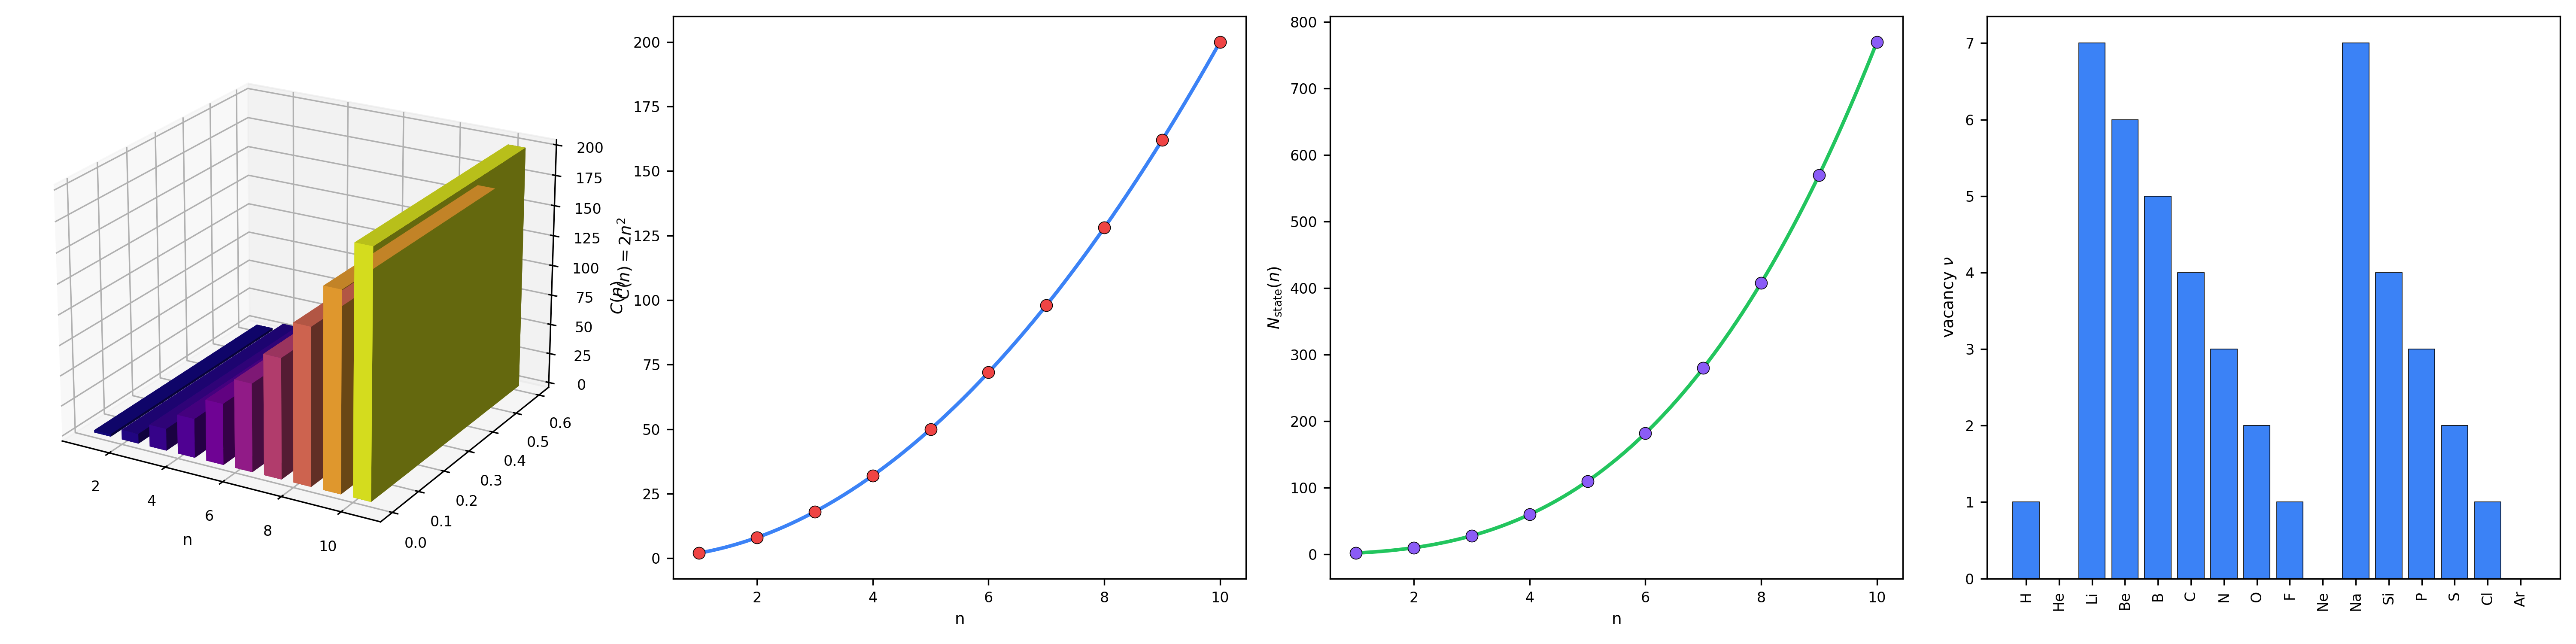
\includegraphics[width=\textwidth]{figures/panel_1_capacity.png}
    \caption{\textbf{Shell Capacity, Cumulative Count, and the Vacancy Ladder.}
    (\textbf{A})~Three-dimensional bar chart of the shell capacity $C(n)=2n^2$ for principal depths $n=1,\ldots,10$, bar height encoding the capacity and colour (plasma scale) tracking its magnitude. The quadratic growth is the derived count $2\sum_{\ell=0}^{n-1}(2\ell+1)=2n^2$ of distinct partition cells at depth $n$, the input the chemical-structure derivation takes from the isolated atom.
    (\textbf{B})~Capacity $C(n)$ on the linear $y$-axis versus depth $n$: the continuous parabola $2n^2$ (blue) with the integer capacities (red points) lying exactly on it for $n=1,\ldots,10$, confirming $C(n)=2n^2$ with no deviation.
    (\textbf{C})~Cumulative partition count $N_{\mathrm{state}}(n)=n(n+1)(2n+1)/3$ (green curve) with the integer cumulative totals (purple points) on the curve, the cubic running sum of the shell capacities.
    (\textbf{D})~Vacancy $\nu=C_v-q_v$ for sixteen elements H through Ar, bars coloured red where $\nu=0$ (closed shell, noble) and blue where $\nu>0$ (open shell). The three red bars are exactly He, Ne, Ar, validating $\nu=0\iff$ noble across all sixteen elements (Theorem~\ref{thm:valence}, Definition~\ref{def:vacancy}).}
    \label{fig:panel_capacity}
\end{figure*}

% ---------------------------------------------------------------------
\begin{figure*}[!htbp]
    \centering
    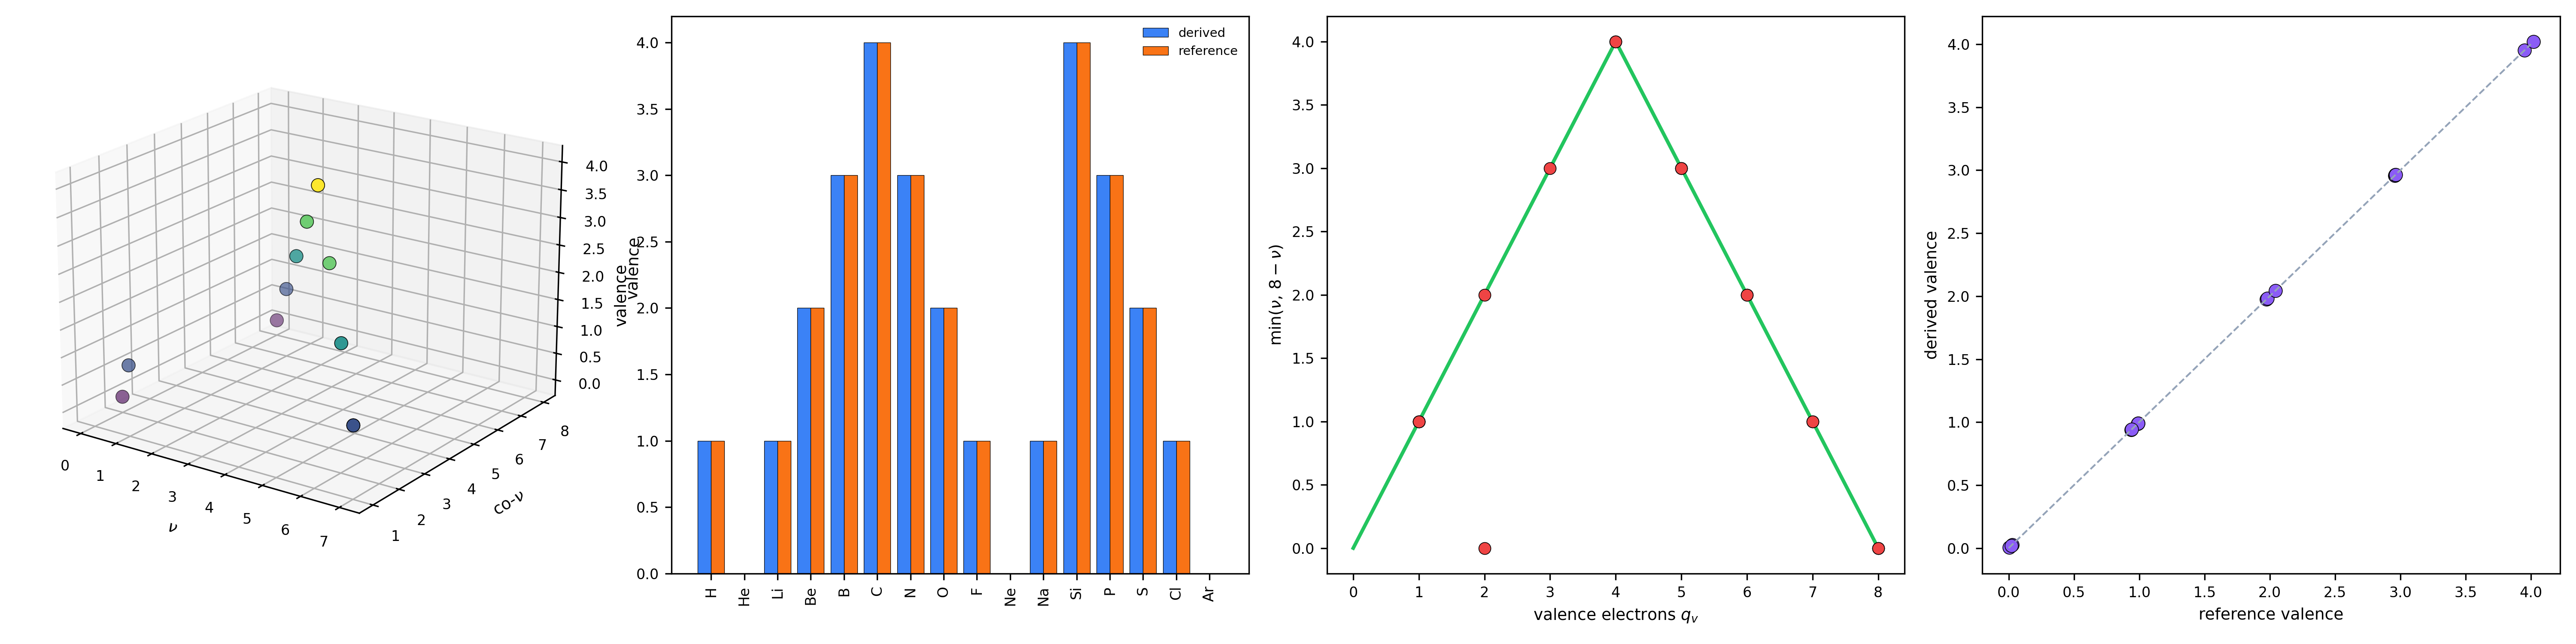
\includegraphics[width=\textwidth]{figures/panel_2_valence.png}
    \caption{\textbf{Valence as the Vacancy Count.}
    (\textbf{A})~Three-dimensional scatter of the sixteen elements in $(\nu,\;C_v-\nu,\;\mathrm{valence})$ space---vacancy against co-vacancy against derived valence---coloured by valence (viridis). The points lie on the surface $\mathrm{valence}=\min(\nu,\,C_v-\nu)$, the covalent-valence rule of Theorem~\ref{thm:valence}.
    (\textbf{B})~Derived valence (blue) and reference common valence (orange) as grouped bars per element. The two series coincide for every element, the $16/16$ agreement of the validation suite.
    (\textbf{C})~The closure curve $\min(\nu,8-\nu)$ (green) over valence-electron count $q_v$, with the elements (red points) sitting on it; the curve peaks at four, recovering carbon's valence of four at $q_v=4$.
    (\textbf{D})~Derived versus reference valence on the identity diagonal (grey dashed); all points lie on the diagonal (small jitter added for visibility), confirming exact reproduction of the common valences from the vacancy arithmetic alone.}
    \label{fig:panel_valence}
\end{figure*}

% ---------------------------------------------------------------------
\begin{figure*}[!htbp]
    \centering
    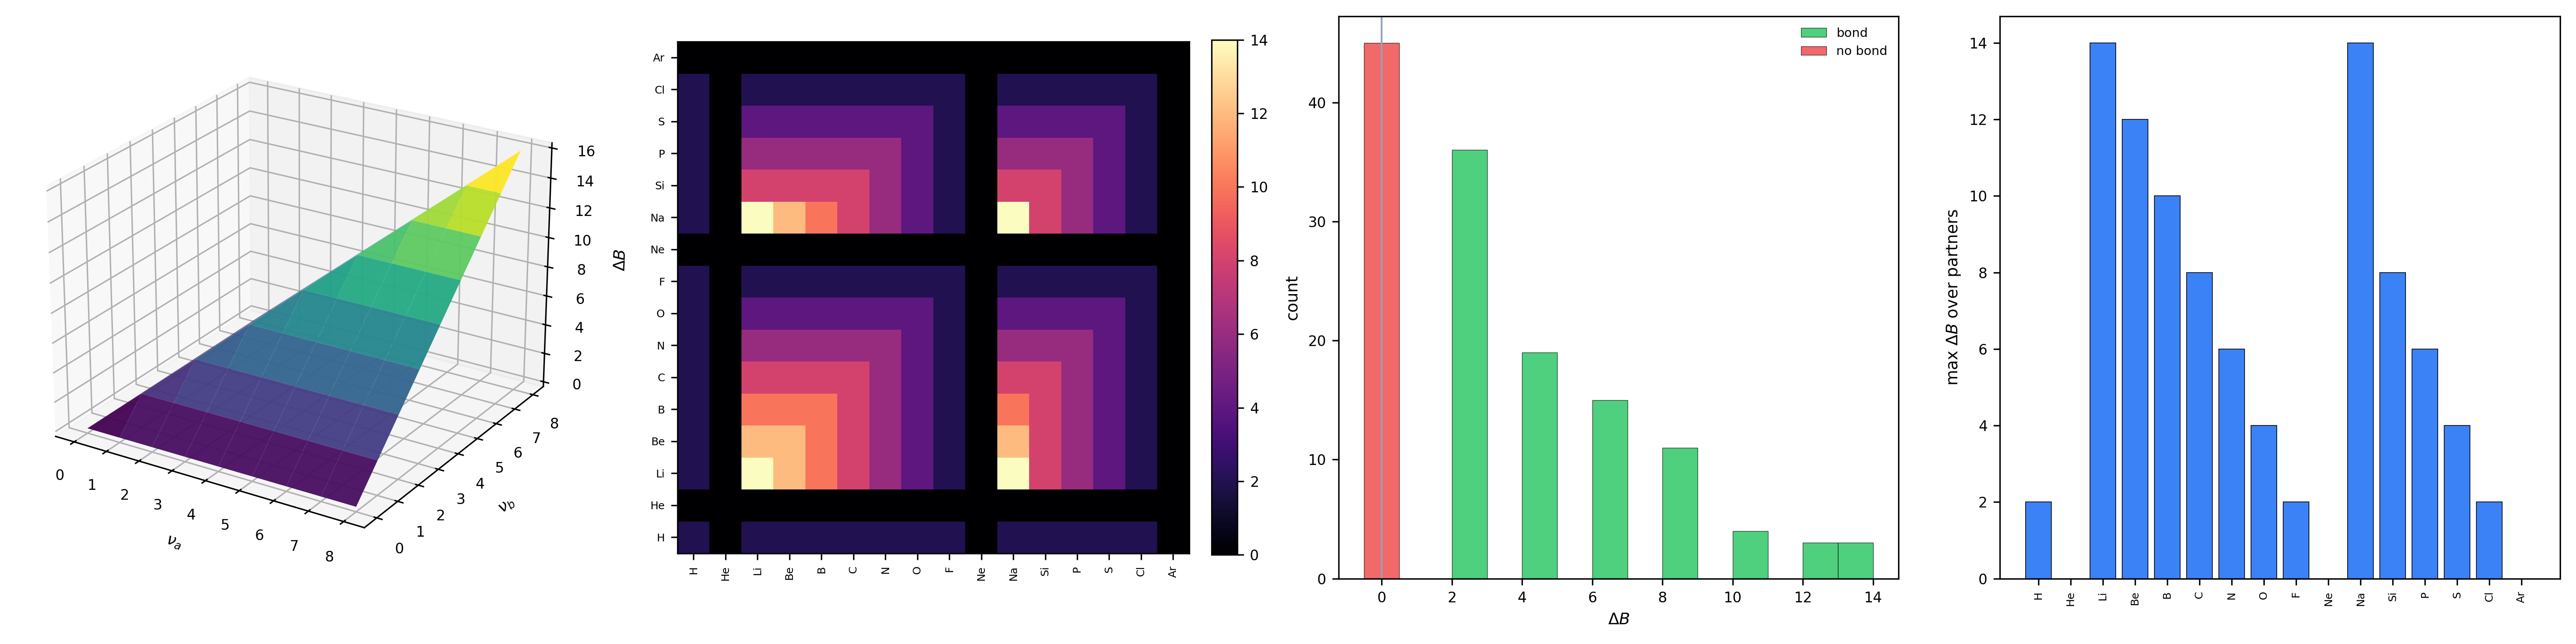
\includegraphics[width=\textwidth]{figures/panel_3_bonding.png}
    \caption{\textbf{The Bonding Criterion over All Element Pairs.}
    (\textbf{A})~Three-dimensional surface of the shared content $\Delta B(\nu_a,\nu_b)$ over the vacancy plane, computed from the monotone thickness model $B=B_0+\kappa\phi(\nu)$ with $\phi(\nu)=\nu$. The surface is positive in the interior and falls to zero along the axes $\nu_a=0$ or $\nu_b=0$: a bond's thickness reduction vanishes whenever either partner is closed-shell (Theorem~\ref{thm:bond}).
    (\textbf{B})~Heatmap of $\Delta B$ across all $136$ element pairs (H through Ar), magma scale. The dark rows and columns are the noble gases He, Ne, Ar, whose shared content is zero with every partner.
    (\textbf{C})~Distribution of $\Delta B$ split into bonding pairs (green, $\Delta B>0$) and non-bonding pairs (red, $\Delta B=0$), separated cleanly about the threshold $\Delta B=0$ (grey line): the sign of $\Delta B$ matches ``neither partner closed-shell'' in all $136$ cases.
    (\textbf{D})~Maximum attainable $\Delta B$ over all partners for each element, bars coloured red for noble (zero) and blue for open-shell. The noble gases alone register zero, the chemical statement that they are inert (Corollary~\ref{cor:noble}).}
    \label{fig:panel_bonding}
\end{figure*}

% ---------------------------------------------------------------------
\begin{figure*}[!htbp]
    \centering
    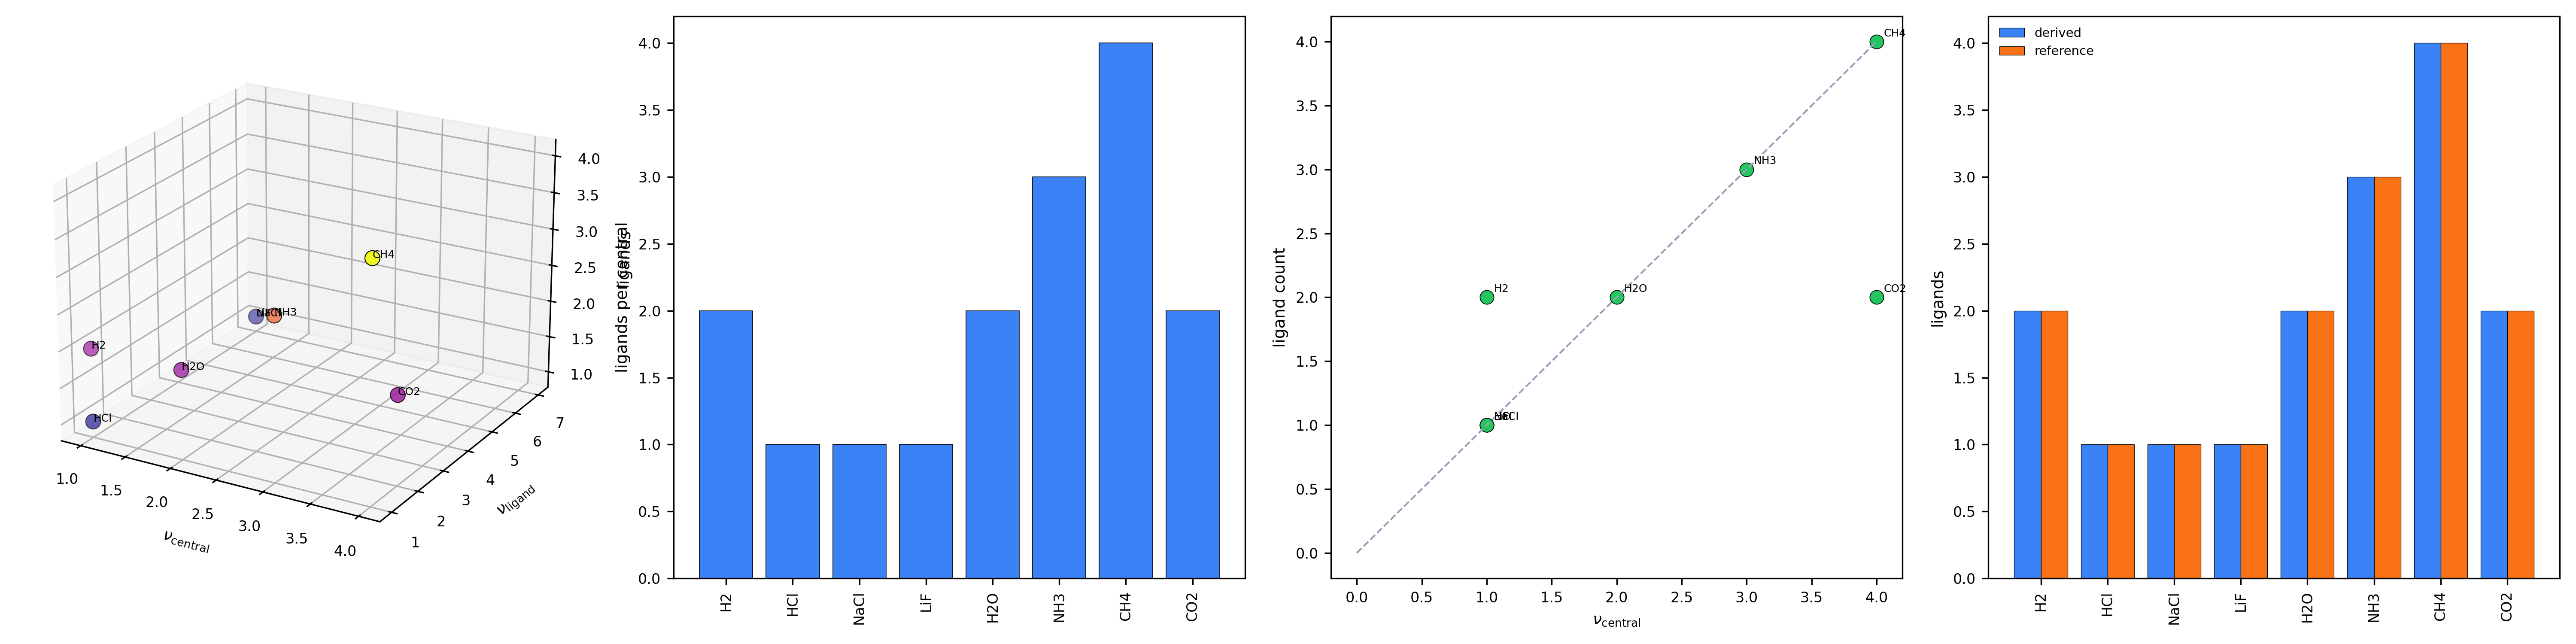
\includegraphics[width=\textwidth]{figures/panel_4_stoichiometry.png}
    \caption{\textbf{Stoichiometry from Vacancy Matching.}
    (\textbf{A})~Three-dimensional scatter of eight molecules in $(\nu_{\mathrm{central}},\,\nu_{\mathrm{ligand}},\,\text{ligand count})$ space, points labelled by molecule and coloured by ligand count (plasma). The ligand count is fixed by closing the central atom's vacancy through interfaces of the ligand's vacancy, recovering the observed formulae.
    (\textbf{B})~Ligands per central atom for H$_2$, HCl, NaCl, LiF, H$_2$O, NH$_3$, CH$_4$, CO$_2$, showing the $1{:}1$, $2{:}1$, $3{:}1$, $4{:}1$ ratios as the central vacancy increases.
    (\textbf{C})~Central vacancy $\nu_{\mathrm{central}}$ versus predicted ligand count; the points track the diagonal (grey dashed) for the hydride series (H$_2$O, NH$_3$, CH$_4$), where each monovalent ligand closes one central vacancy.
    (\textbf{D})~Derived (blue) versus reference (orange) ligand count per molecule as grouped bars; the two coincide for all eight molecules ($8/8$), the vacancy ratio reproducing each stoichiometry with no further input.}
    \label{fig:panel_stoichiometry}
\end{figure*}

% ---------------------------------------------------------------------
\begin{figure*}[!htbp]
    \centering
    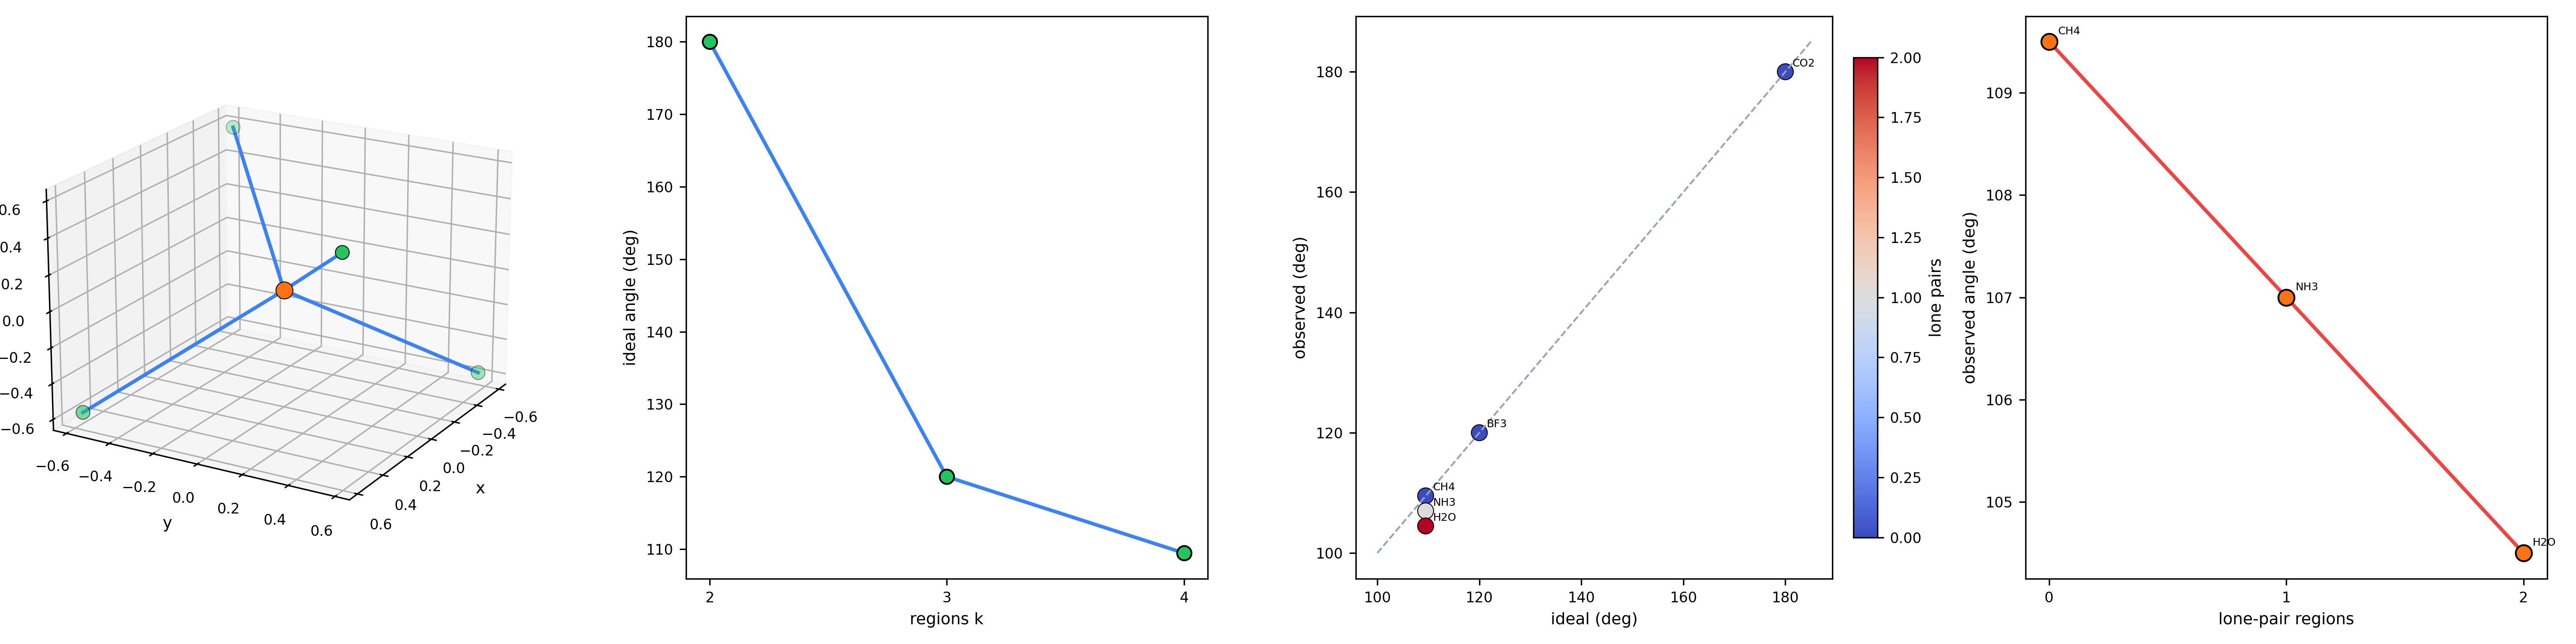
\includegraphics[width=\textwidth]{figures/panel_5_geometry.png}
    \caption{\textbf{Molecular Geometry as Maximal Angular Separation.}
    (\textbf{A})~Three-dimensional rendering of the four maximally separated bond directions of a four-coordinate centre (methane): bonds (blue) from the central atom (orange) to the four ligand directions (green) at the regular-tetrahedron vertices, the configuration that minimises pairwise solid-angle overlap (Theorem~\ref{thm:geometry}).
    (\textbf{B})~Ideal symmetric bond angle versus number of interface regions $k$: $180^\circ$ ($k=2$, linear), $120^\circ$ ($k=3$, trigonal planar), $109.47^\circ$ ($k=4$, tetrahedral)---the maximal-separation angles of $k$ points on the sphere.
    (\textbf{C})~Observed versus ideal symmetric angle for five molecules, coloured by lone-pair count (coolwarm); points on the diagonal (grey dashed) are the lone-pair-free backbones (CO$_2$, BF$_3$, CH$_4$), and points below it are the lone-pair-compressed geometries (NH$_3$, H$_2$O).
    (\textbf{D})~Observed angle of the four-region family versus lone-pair count: $109.5^\circ$ (CH$_4$, none) $\to 107^\circ$ (NH$_3$, one) $\to 104.5^\circ$ (H$_2$O, two), the monotone compression as unshared regions are added.}
    \label{fig:panel_geometry}
\end{figure*}

% ---------------------------------------------------------------------
\begin{figure*}[!htbp]
    \centering
    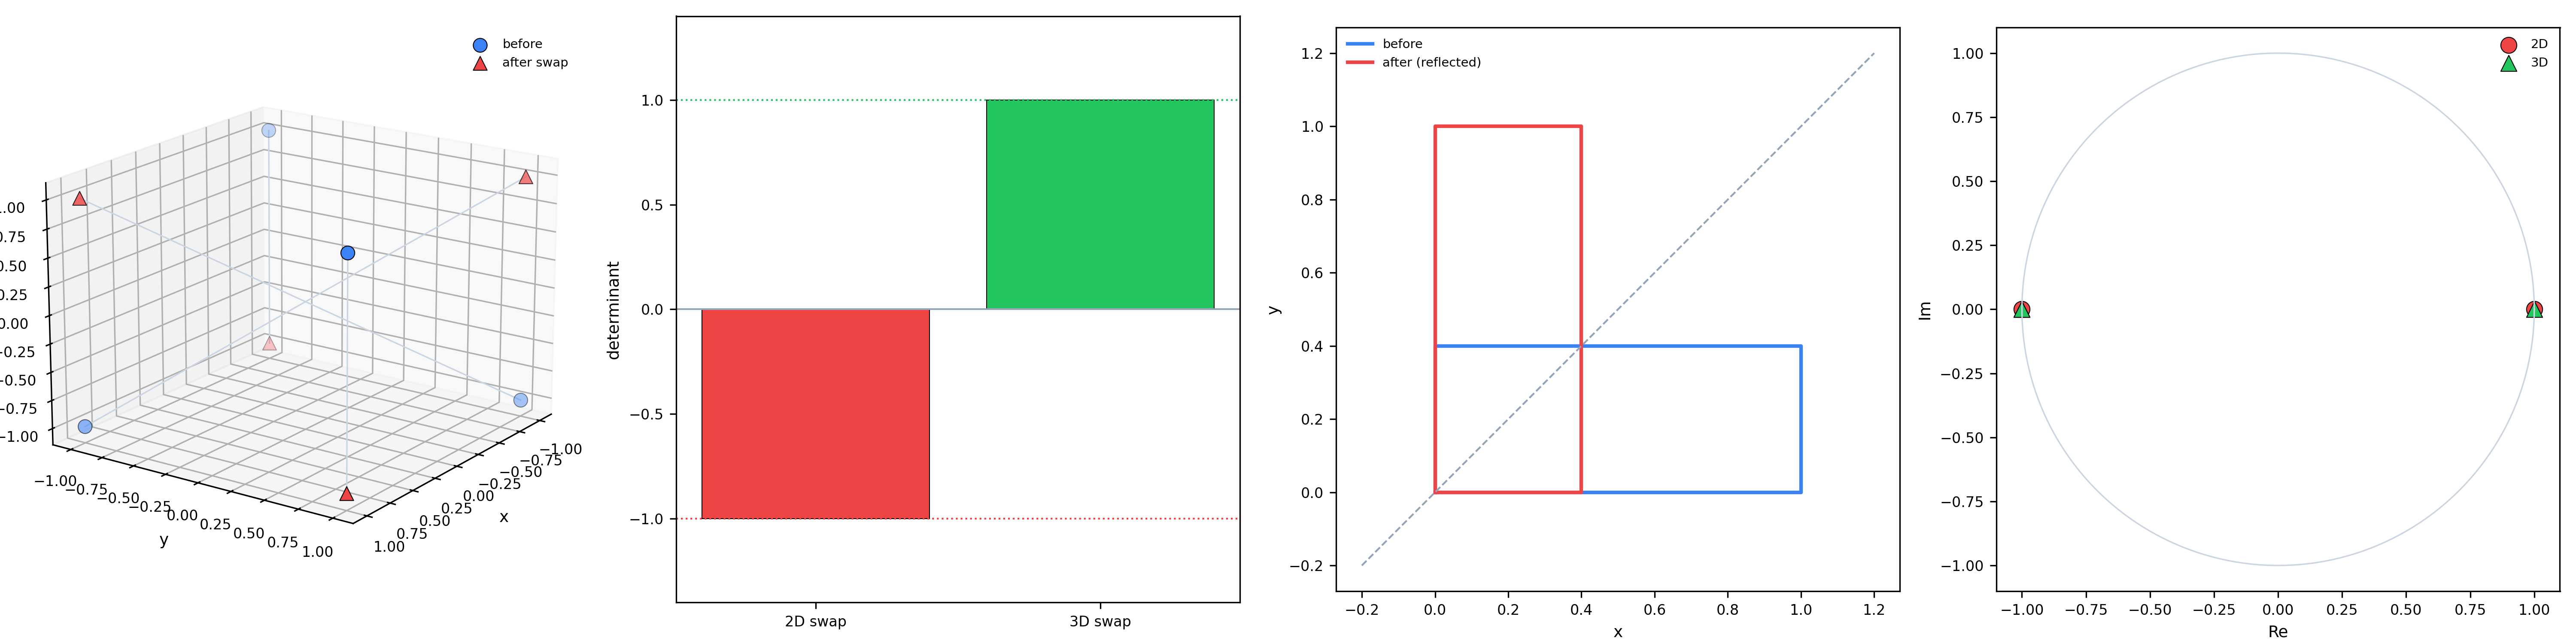
\includegraphics[width=\textwidth]{figures/panel_6_dimension.png}
    \caption{\textbf{Three Dimensions and the Absence of a Privileged Axis.}
    (\textbf{A})~Three-dimensional action of the axis-swap $(x,y,z)\mapsto(y,x,-z)$ on the vertices of a tetrahedron: original vertices (blue) and their images (red triangles) joined by displacement lines. The swap is realised as a continuous proper rotation, exchanging the two axes by an internal motion (Principle~\ref{prin:threed}).
    (\textbf{B})~Determinants of the axis-swap matrices: the two-dimensional swap has determinant $-1$ (a reflection, red) and the three-dimensional swap has determinant $+1$ (a proper rotation in $SO(3)$, green), the dashed guides marking $\pm1$.
    (\textbf{C})~The two-dimensional swap as a reflection across the line $y=x$ (grey dashed): a rectangle (blue) mapped to its mirror image (red), showing that in $d=2$ exchanging the axes requires a reflection, not an internal rotation---hence an external choice.
    (\textbf{D})~Eigenvalue spectra of the two swap matrices on the unit circle (grey): the two-dimensional swap (red) has eigenvalues $\pm1$, the three-dimensional swap (green triangles) has eigenvalues consistent with a proper rotation, confirming $d=3$ as the minimum dimension of selector-free axis exchange.}
    \label{fig:panel_dimension}
\end{figure*}

% ---------------------------------------------------------------------
\begin{figure*}[!htbp]
    \centering
    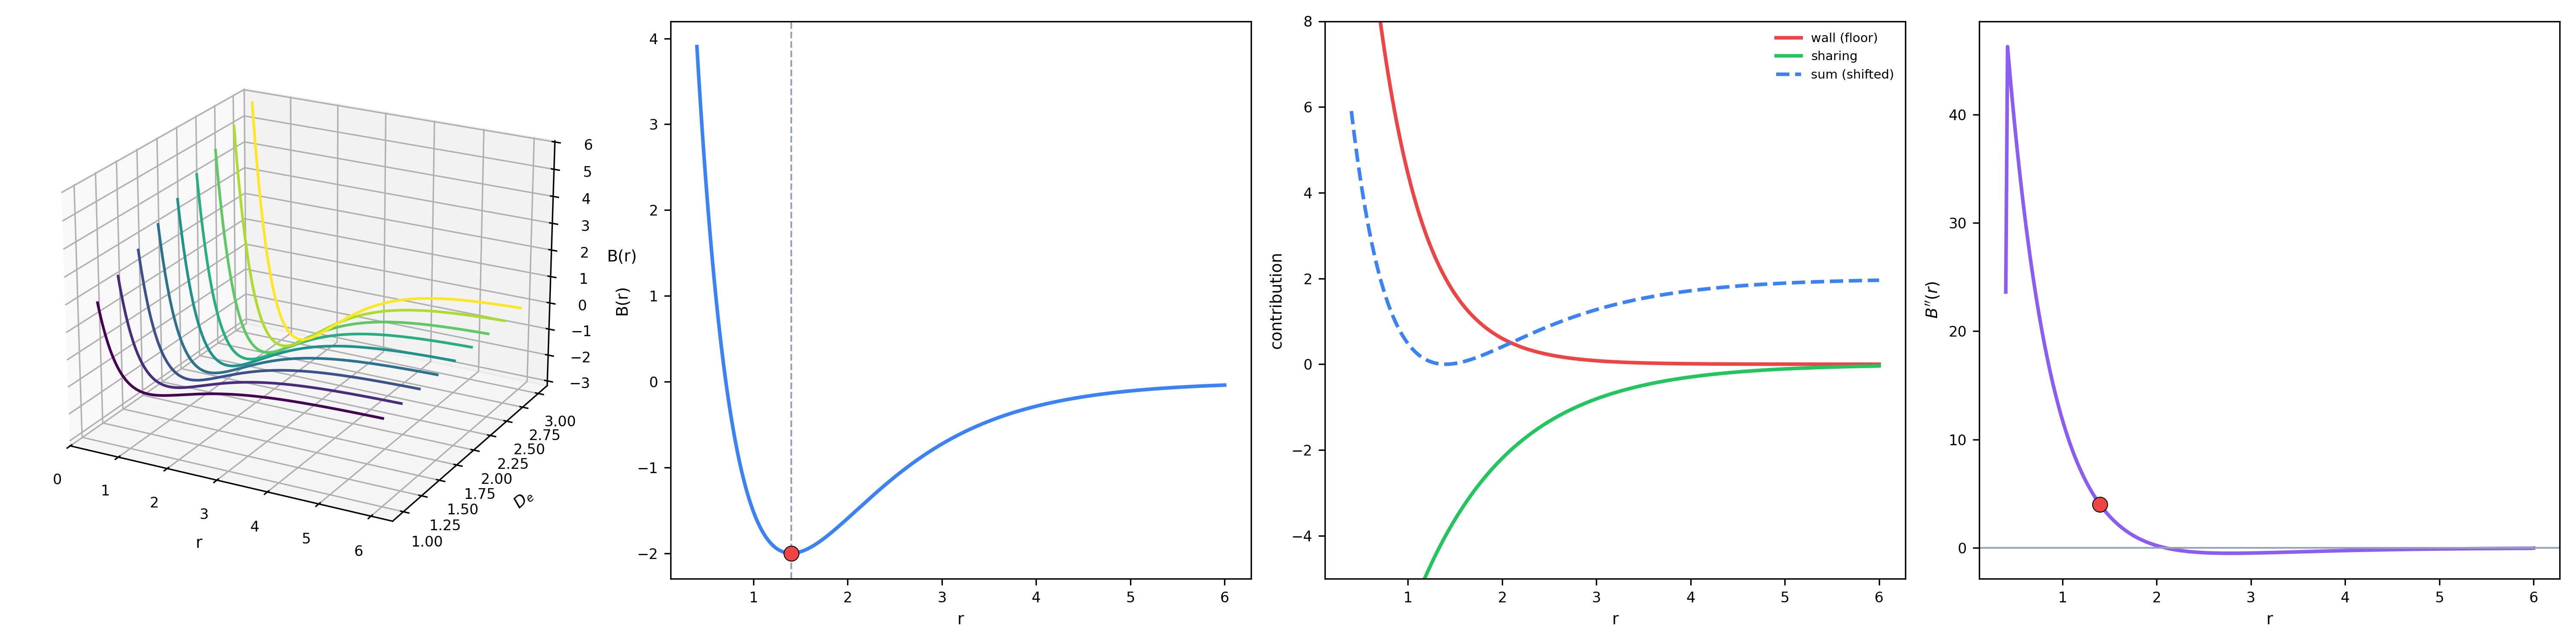
\includegraphics[width=\textwidth]{figures/panel_7_bondlength.png}
    \caption{\textbf{Bond Length as the Convex Thickness Minimiser.}
    (\textbf{A})~Three-dimensional family of joint-thickness wells $B(r)=D_e[(1-e^{-d(r-r_0)})^2-1]$ over internuclear separation $r$ and well depth $D_e$ (viridis), each curve a convex well with a single interior minimum; the minimum deepens with $D_e$ but never moves to $r=0$.
    (\textbf{B})~The thickness profile $B(r)$ (blue) with its unique interior minimiser marked (red point at $r^{*}=1.40$, in units of $r_0$); the dashed line locates $r^{*}$. The curve diverges as $r\to0$ and plateaus as $r\to\infty$, the equilibrium standoff of Theorem~\ref{thm:length}.
    (\textbf{C})~The two competing contributions: the repulsive wall (red, diverging as $r\to0$---the contact floor asserting itself), the sharing pull (green, the boundary-reduction drawing the atoms together), and their sum (blue dashed) with the interior minimum, showing the floor as the origin of short-range repulsion.
    (\textbf{D})~Curvature $B''(r)$ (purple) versus separation; it is positive at the minimiser (red point) and crosses zero only well away from it, confirming the well is locally convex at $r^{*}$ ($B''(r^{*})=3.99>0$).}
    \label{fig:panel_bondlength}
\end{figure*}

% ---------------------------------------------------------------------
\begin{figure*}[!htbp]
    \centering
    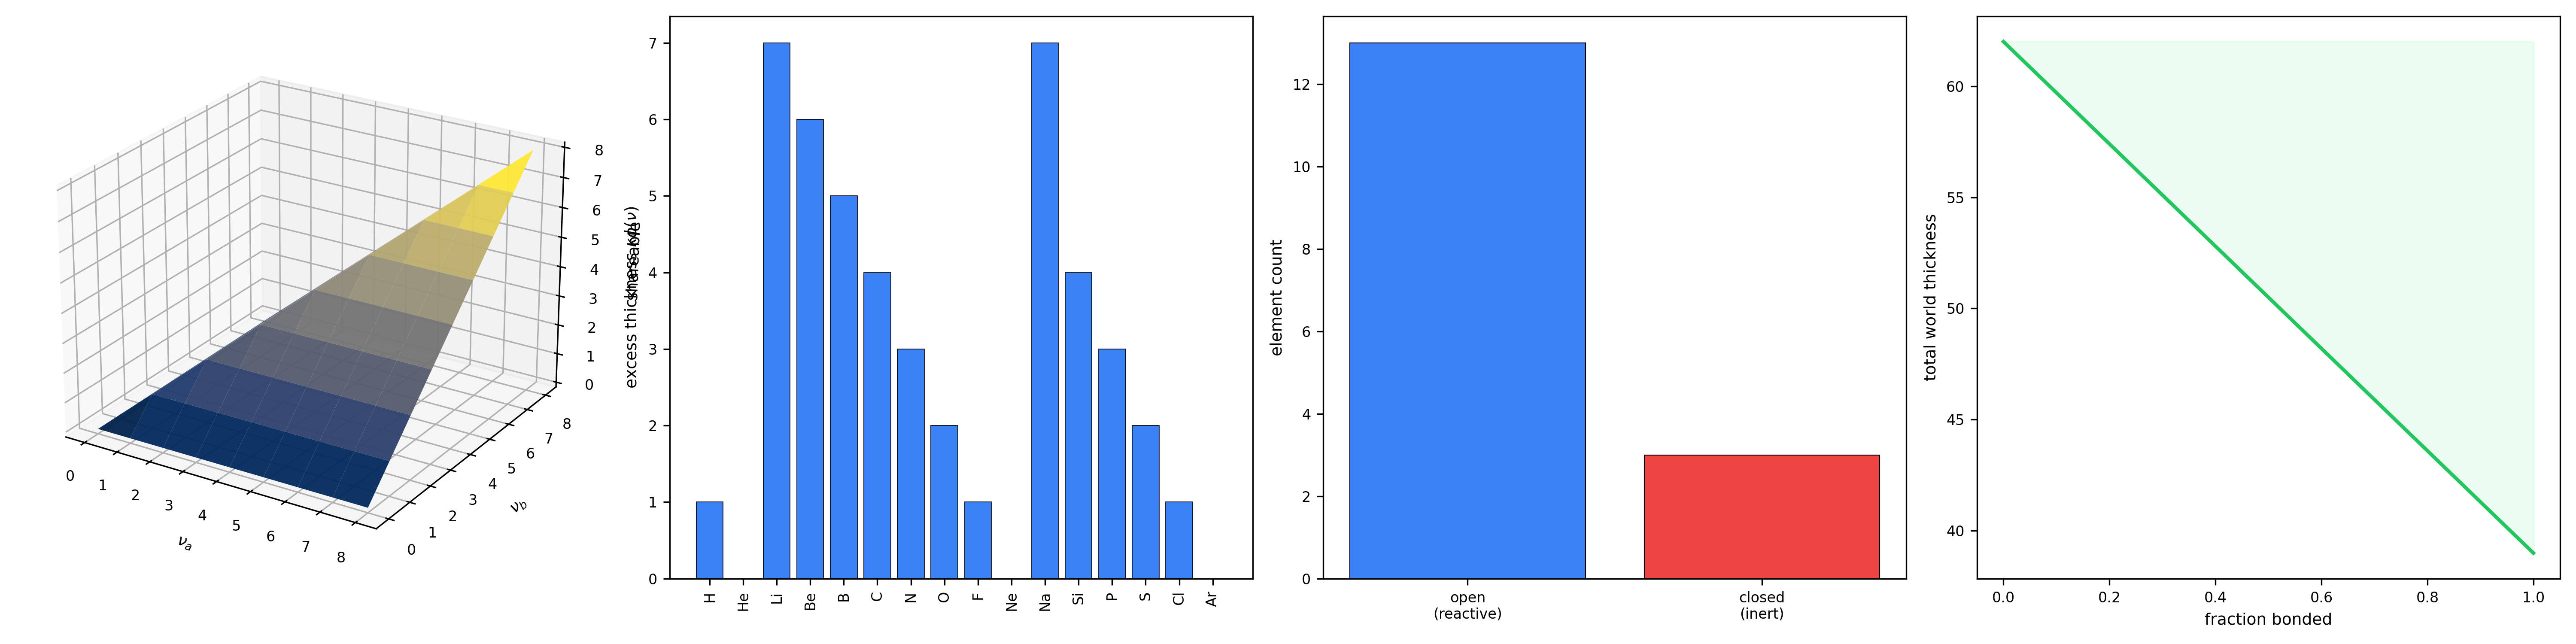
\includegraphics[width=\textwidth]{figures/panel_8_existence.png}
    \caption{\textbf{Why a World of Bounded Atoms Must Be a World of Molecules.}
    (\textbf{A})~Three-dimensional surface of the shareable content $\min(\nu_a,\nu_b)$ over the vacancy plane (cividis): the boundary that two atoms can commit jointly, zero whenever either is closed-shell and rising with the smaller vacancy, the resource from which structure is built.
    (\textbf{B})~Excess boundary thickness $\kappa\phi(\nu)$ above the closed-shell minimum for sixteen elements, bars red where $\nu=0$ (no excess: the noble-gas minimum) and blue where $\nu>0$ (excess to be relaxed by bonding).
    (\textbf{C})~Element census of the open (reactive, blue) versus closed (inert, red) shells among the sixteen elements, the count of atoms that carry shareable vacancy versus those that do not.
    (\textbf{D})~Total world boundary thickness versus the fraction of open atoms that have bonded: the monotone decrease (green, shaded reduction) shows that a world of bounded atoms with positive vacancy lowers its total thickness by forming molecules---chemical structure as the floor's economy (Theorem~\ref{thm:why}).}
    \label{fig:panel_existence}
\end{figure*}
 or copy individually.
% =====================================================================

% ---------------------------------------------------------------------
\begin{figure*}[!htbp]
    \centering
    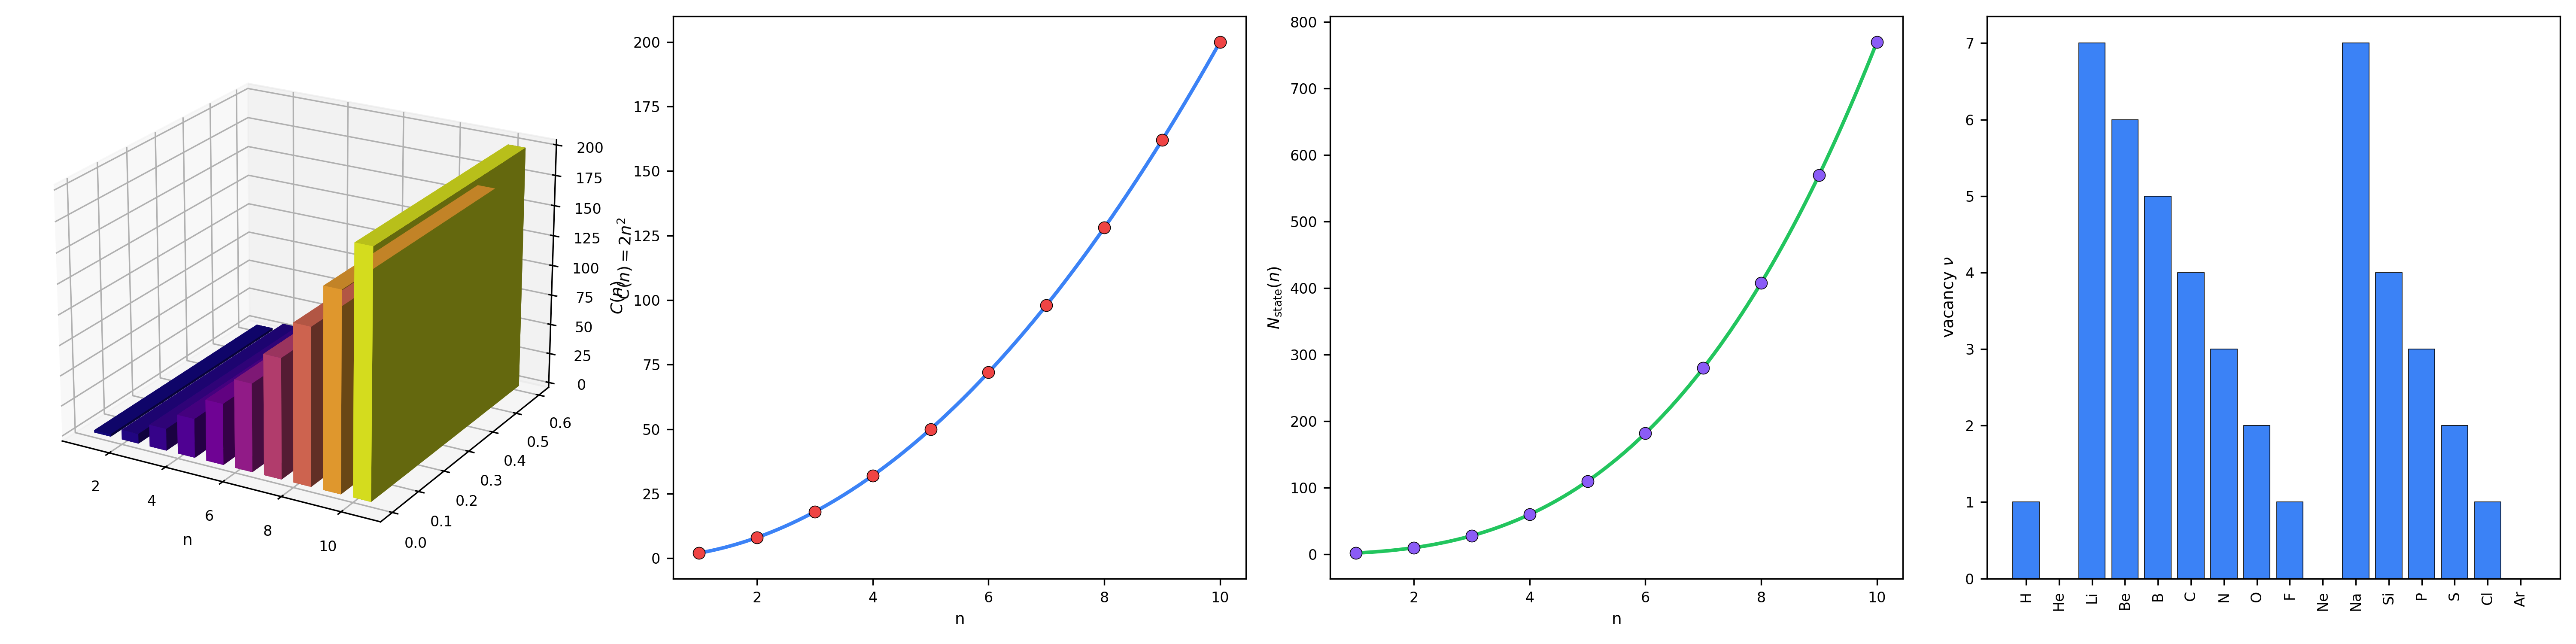
\includegraphics[width=\textwidth]{figures/panel_1_capacity.png}
    \caption{\textbf{Shell Capacity, Cumulative Count, and the Vacancy Ladder.}
    (\textbf{A})~Three-dimensional bar chart of the shell capacity $C(n)=2n^2$ for principal depths $n=1,\ldots,10$, bar height encoding the capacity and colour (plasma scale) tracking its magnitude. The quadratic growth is the derived count $2\sum_{\ell=0}^{n-1}(2\ell+1)=2n^2$ of distinct partition cells at depth $n$, the input the chemical-structure derivation takes from the isolated atom.
    (\textbf{B})~Capacity $C(n)$ on the linear $y$-axis versus depth $n$: the continuous parabola $2n^2$ (blue) with the integer capacities (red points) lying exactly on it for $n=1,\ldots,10$, confirming $C(n)=2n^2$ with no deviation.
    (\textbf{C})~Cumulative partition count $N_{\mathrm{state}}(n)=n(n+1)(2n+1)/3$ (green curve) with the integer cumulative totals (purple points) on the curve, the cubic running sum of the shell capacities.
    (\textbf{D})~Vacancy $\nu=C_v-q_v$ for sixteen elements H through Ar, bars coloured red where $\nu=0$ (closed shell, noble) and blue where $\nu>0$ (open shell). The three red bars are exactly He, Ne, Ar, validating $\nu=0\iff$ noble across all sixteen elements (Theorem~\ref{thm:valence}, Definition~\ref{def:vacancy}).}
    \label{fig:panel_capacity}
\end{figure*}

% ---------------------------------------------------------------------
\begin{figure*}[!htbp]
    \centering
    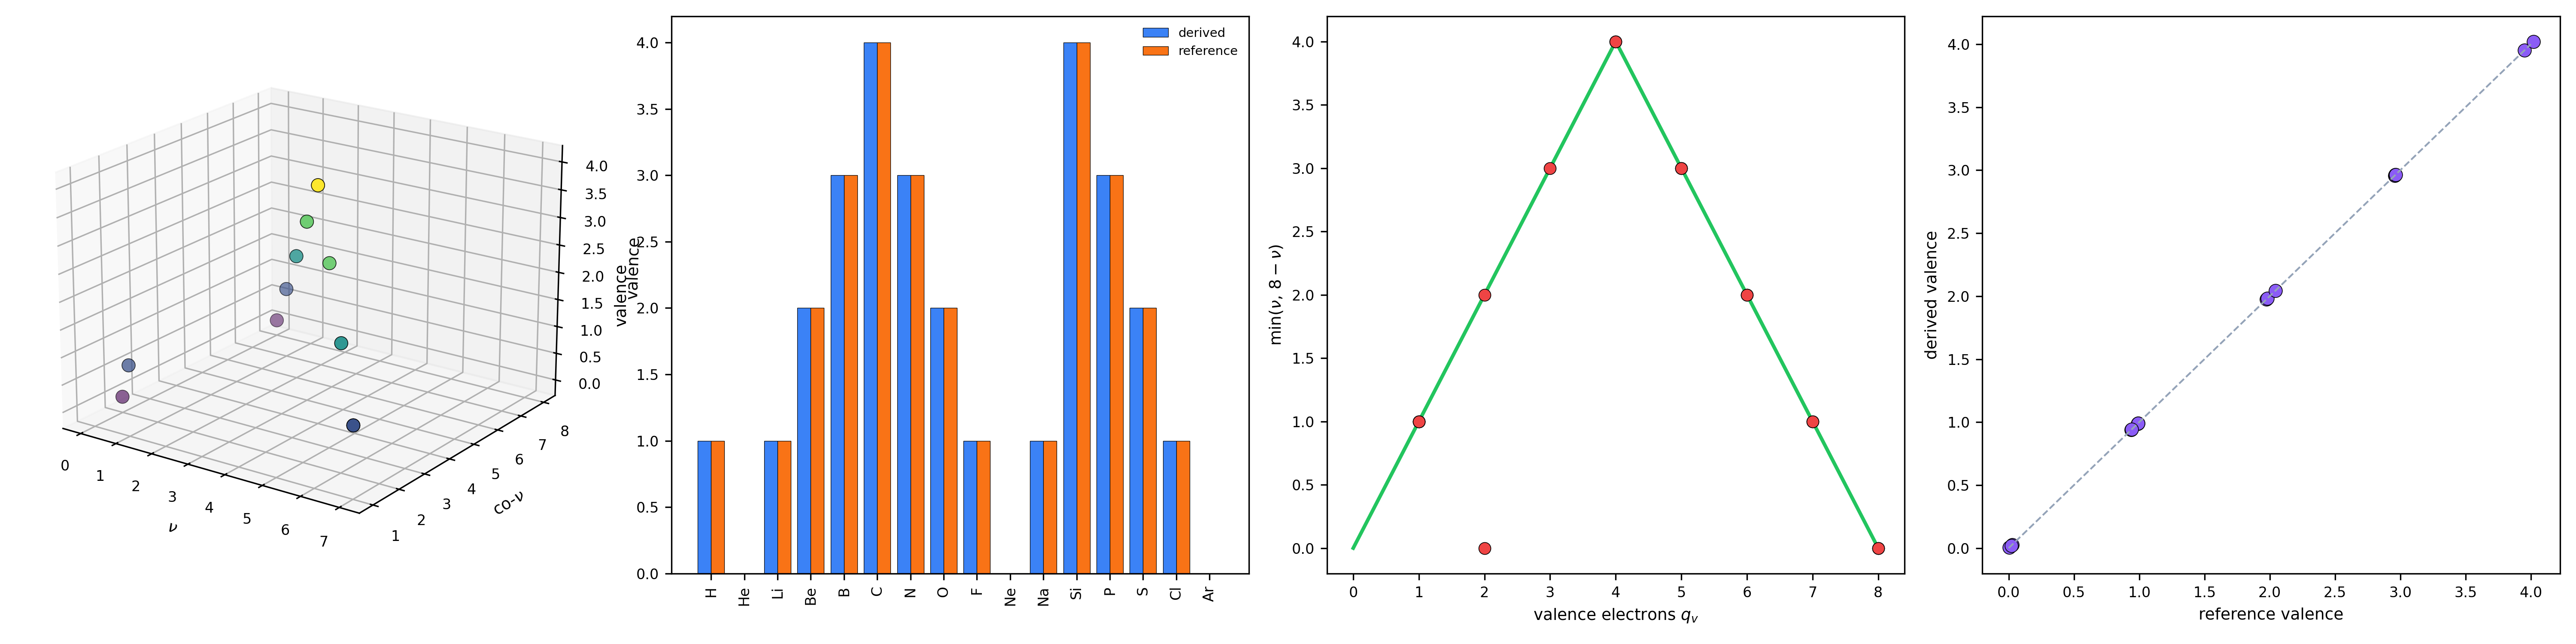
\includegraphics[width=\textwidth]{figures/panel_2_valence.png}
    \caption{\textbf{Valence as the Vacancy Count.}
    (\textbf{A})~Three-dimensional scatter of the sixteen elements in $(\nu,\;C_v-\nu,\;\mathrm{valence})$ space---vacancy against co-vacancy against derived valence---coloured by valence (viridis). The points lie on the surface $\mathrm{valence}=\min(\nu,\,C_v-\nu)$, the covalent-valence rule of Theorem~\ref{thm:valence}.
    (\textbf{B})~Derived valence (blue) and reference common valence (orange) as grouped bars per element. The two series coincide for every element, the $16/16$ agreement of the validation suite.
    (\textbf{C})~The closure curve $\min(\nu,8-\nu)$ (green) over valence-electron count $q_v$, with the elements (red points) sitting on it; the curve peaks at four, recovering carbon's valence of four at $q_v=4$.
    (\textbf{D})~Derived versus reference valence on the identity diagonal (grey dashed); all points lie on the diagonal (small jitter added for visibility), confirming exact reproduction of the common valences from the vacancy arithmetic alone.}
    \label{fig:panel_valence}
\end{figure*}

% ---------------------------------------------------------------------
\begin{figure*}[!htbp]
    \centering
    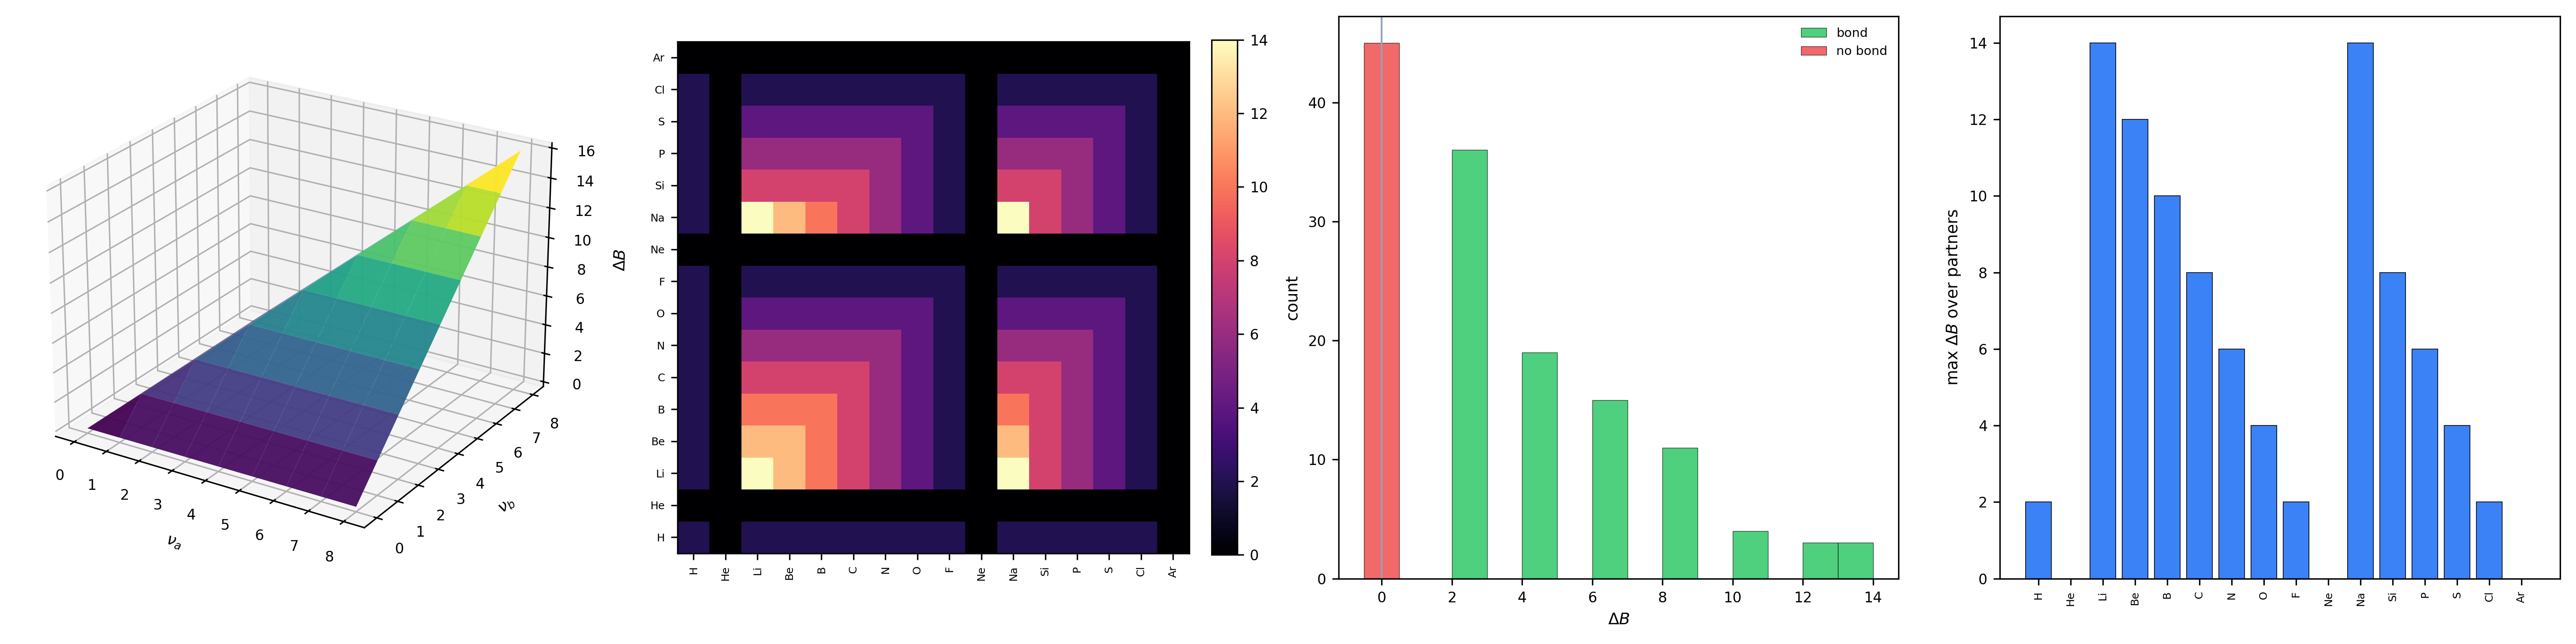
\includegraphics[width=\textwidth]{figures/panel_3_bonding.png}
    \caption{\textbf{The Bonding Criterion over All Element Pairs.}
    (\textbf{A})~Three-dimensional surface of the shared content $\Delta B(\nu_a,\nu_b)$ over the vacancy plane, computed from the monotone thickness model $B=B_0+\kappa\phi(\nu)$ with $\phi(\nu)=\nu$. The surface is positive in the interior and falls to zero along the axes $\nu_a=0$ or $\nu_b=0$: a bond's thickness reduction vanishes whenever either partner is closed-shell (Theorem~\ref{thm:bond}).
    (\textbf{B})~Heatmap of $\Delta B$ across all $136$ element pairs (H through Ar), magma scale. The dark rows and columns are the noble gases He, Ne, Ar, whose shared content is zero with every partner.
    (\textbf{C})~Distribution of $\Delta B$ split into bonding pairs (green, $\Delta B>0$) and non-bonding pairs (red, $\Delta B=0$), separated cleanly about the threshold $\Delta B=0$ (grey line): the sign of $\Delta B$ matches ``neither partner closed-shell'' in all $136$ cases.
    (\textbf{D})~Maximum attainable $\Delta B$ over all partners for each element, bars coloured red for noble (zero) and blue for open-shell. The noble gases alone register zero, the chemical statement that they are inert (Corollary~\ref{cor:noble}).}
    \label{fig:panel_bonding}
\end{figure*}

% ---------------------------------------------------------------------
\begin{figure*}[!htbp]
    \centering
    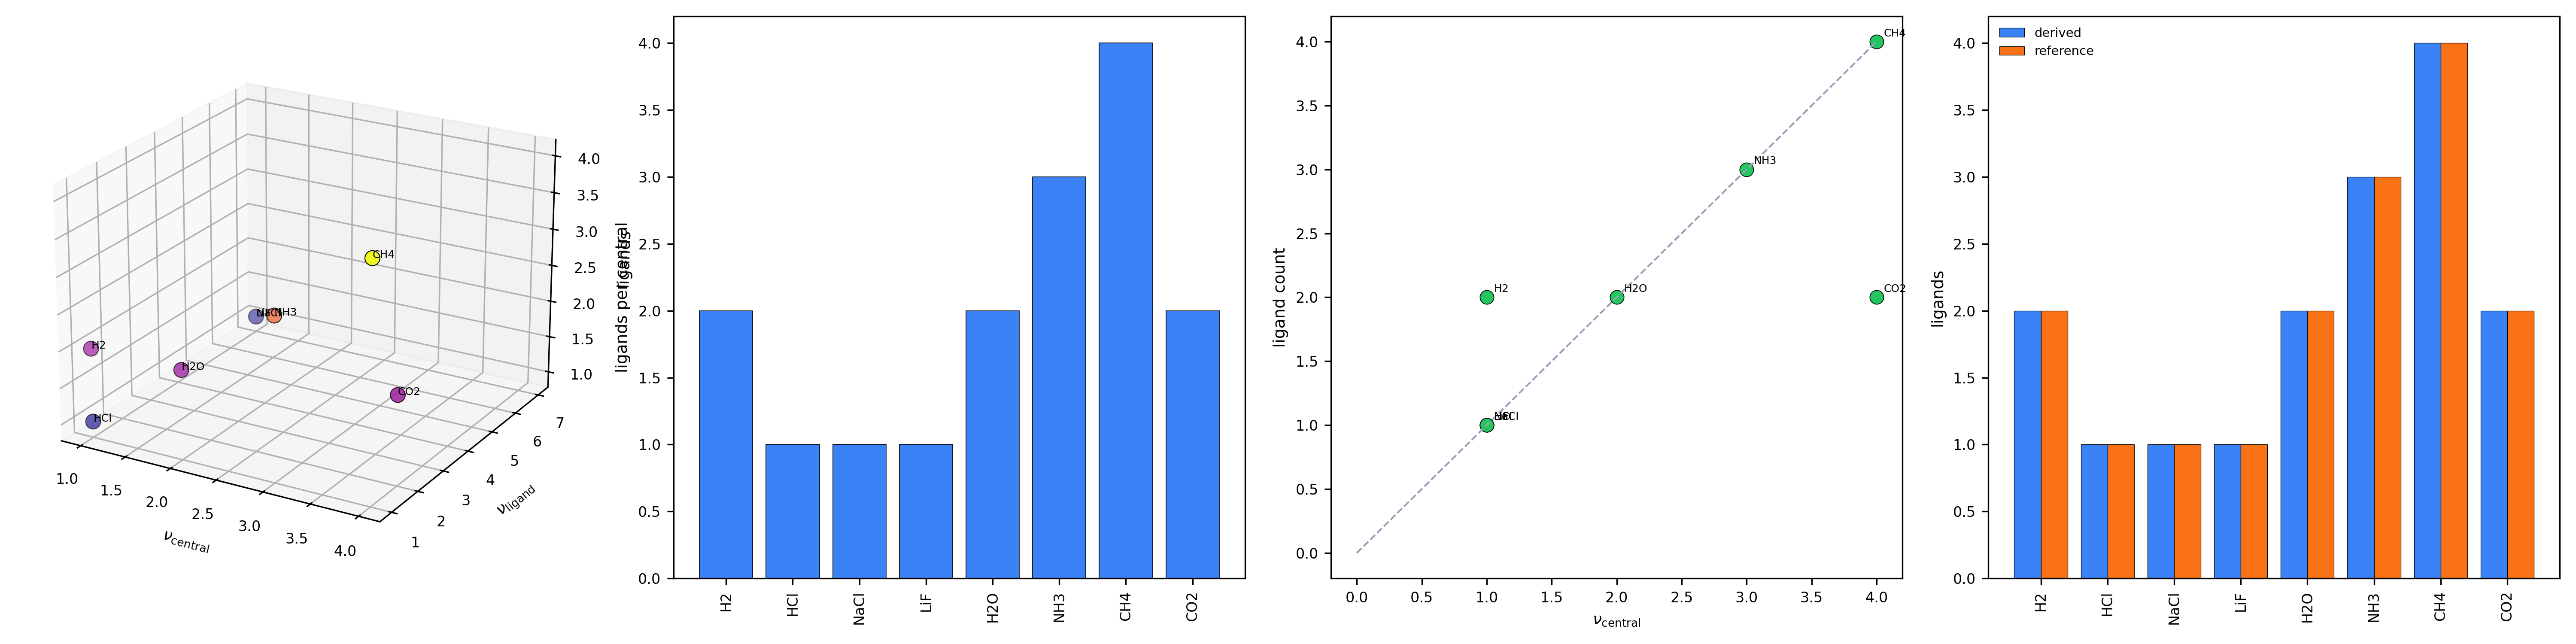
\includegraphics[width=\textwidth]{figures/panel_4_stoichiometry.png}
    \caption{\textbf{Stoichiometry from Vacancy Matching.}
    (\textbf{A})~Three-dimensional scatter of eight molecules in $(\nu_{\mathrm{central}},\,\nu_{\mathrm{ligand}},\,\text{ligand count})$ space, points labelled by molecule and coloured by ligand count (plasma). The ligand count is fixed by closing the central atom's vacancy through interfaces of the ligand's vacancy, recovering the observed formulae.
    (\textbf{B})~Ligands per central atom for H$_2$, HCl, NaCl, LiF, H$_2$O, NH$_3$, CH$_4$, CO$_2$, showing the $1{:}1$, $2{:}1$, $3{:}1$, $4{:}1$ ratios as the central vacancy increases.
    (\textbf{C})~Central vacancy $\nu_{\mathrm{central}}$ versus predicted ligand count; the points track the diagonal (grey dashed) for the hydride series (H$_2$O, NH$_3$, CH$_4$), where each monovalent ligand closes one central vacancy.
    (\textbf{D})~Derived (blue) versus reference (orange) ligand count per molecule as grouped bars; the two coincide for all eight molecules ($8/8$), the vacancy ratio reproducing each stoichiometry with no further input.}
    \label{fig:panel_stoichiometry}
\end{figure*}

% ---------------------------------------------------------------------
\begin{figure*}[!htbp]
    \centering
    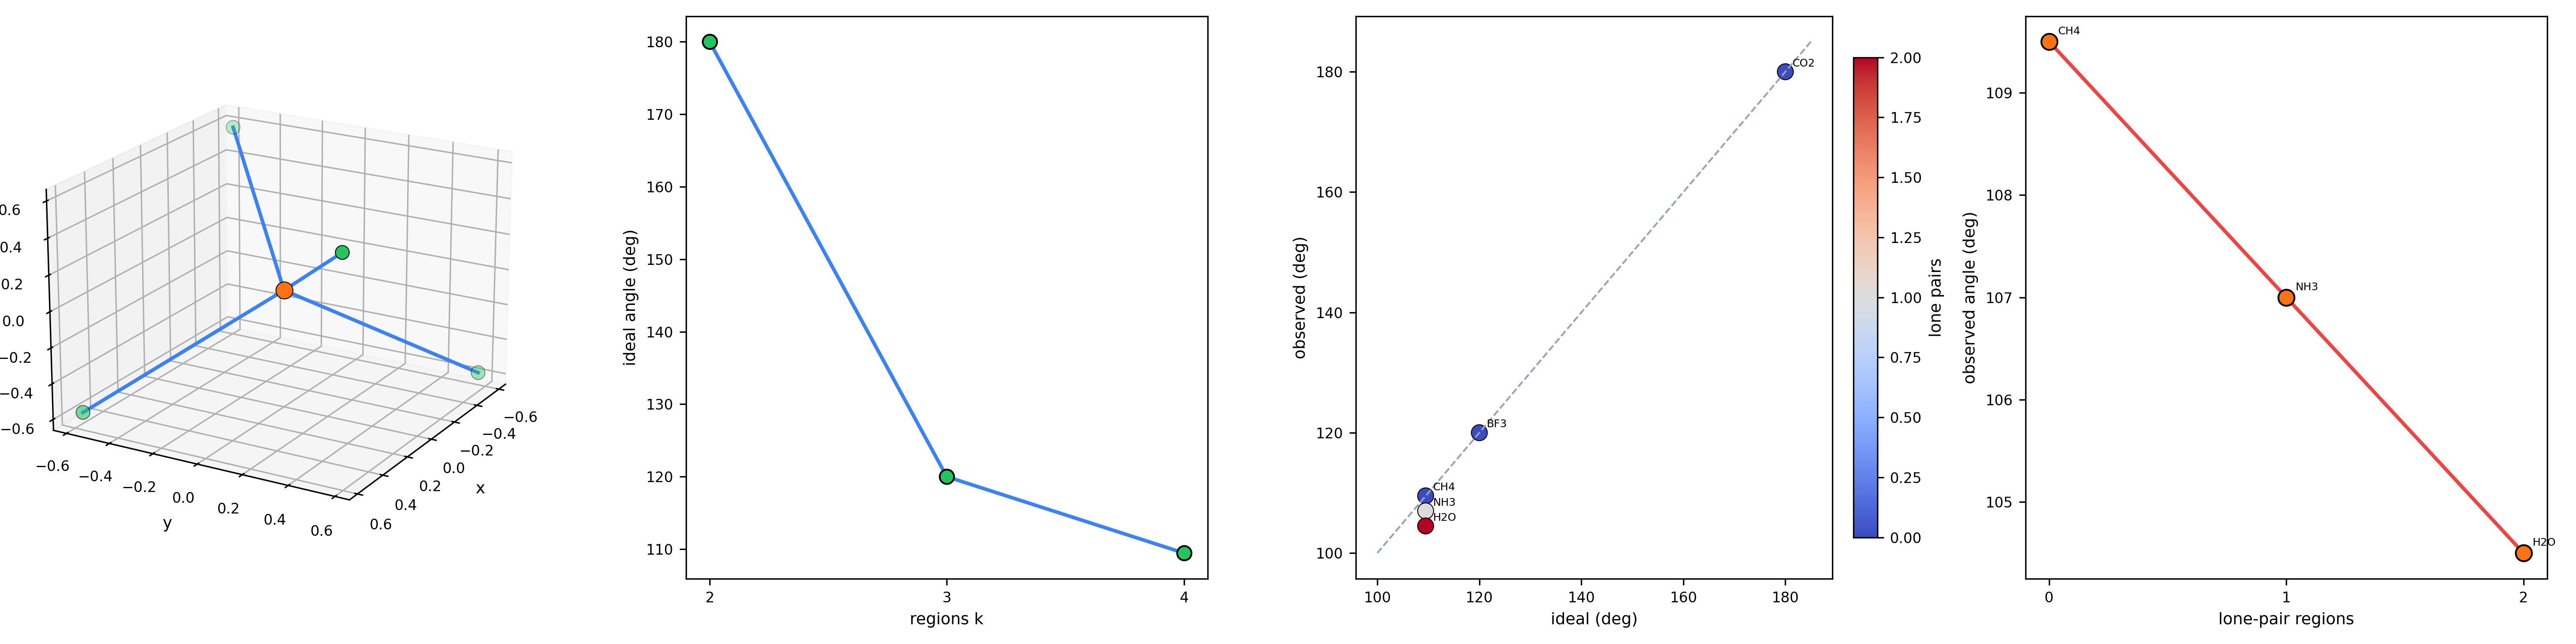
\includegraphics[width=\textwidth]{figures/panel_5_geometry.png}
    \caption{\textbf{Molecular Geometry as Maximal Angular Separation.}
    (\textbf{A})~Three-dimensional rendering of the four maximally separated bond directions of a four-coordinate centre (methane): bonds (blue) from the central atom (orange) to the four ligand directions (green) at the regular-tetrahedron vertices, the configuration that minimises pairwise solid-angle overlap (Theorem~\ref{thm:geometry}).
    (\textbf{B})~Ideal symmetric bond angle versus number of interface regions $k$: $180^\circ$ ($k=2$, linear), $120^\circ$ ($k=3$, trigonal planar), $109.47^\circ$ ($k=4$, tetrahedral)---the maximal-separation angles of $k$ points on the sphere.
    (\textbf{C})~Observed versus ideal symmetric angle for five molecules, coloured by lone-pair count (coolwarm); points on the diagonal (grey dashed) are the lone-pair-free backbones (CO$_2$, BF$_3$, CH$_4$), and points below it are the lone-pair-compressed geometries (NH$_3$, H$_2$O).
    (\textbf{D})~Observed angle of the four-region family versus lone-pair count: $109.5^\circ$ (CH$_4$, none) $\to 107^\circ$ (NH$_3$, one) $\to 104.5^\circ$ (H$_2$O, two), the monotone compression as unshared regions are added.}
    \label{fig:panel_geometry}
\end{figure*}

% ---------------------------------------------------------------------
\begin{figure*}[!htbp]
    \centering
    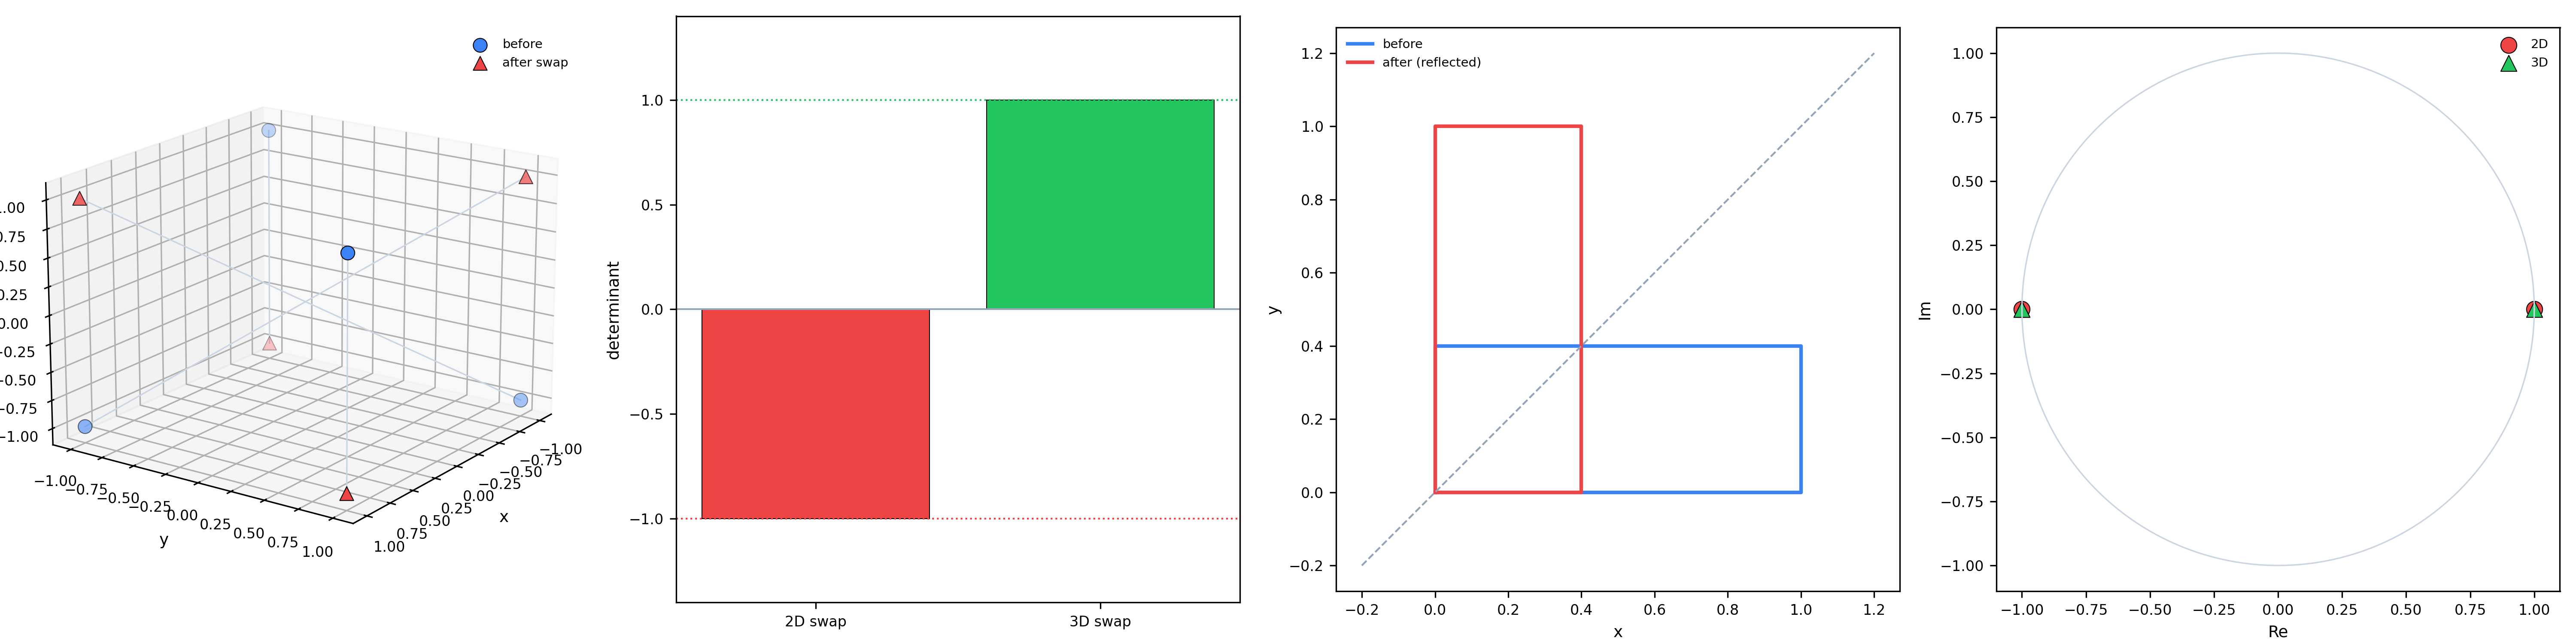
\includegraphics[width=\textwidth]{figures/panel_6_dimension.png}
    \caption{\textbf{Three Dimensions and the Absence of a Privileged Axis.}
    (\textbf{A})~Three-dimensional action of the axis-swap $(x,y,z)\mapsto(y,x,-z)$ on the vertices of a tetrahedron: original vertices (blue) and their images (red triangles) joined by displacement lines. The swap is realised as a continuous proper rotation, exchanging the two axes by an internal motion (Principle~\ref{prin:threed}).
    (\textbf{B})~Determinants of the axis-swap matrices: the two-dimensional swap has determinant $-1$ (a reflection, red) and the three-dimensional swap has determinant $+1$ (a proper rotation in $SO(3)$, green), the dashed guides marking $\pm1$.
    (\textbf{C})~The two-dimensional swap as a reflection across the line $y=x$ (grey dashed): a rectangle (blue) mapped to its mirror image (red), showing that in $d=2$ exchanging the axes requires a reflection, not an internal rotation---hence an external choice.
    (\textbf{D})~Eigenvalue spectra of the two swap matrices on the unit circle (grey): the two-dimensional swap (red) has eigenvalues $\pm1$, the three-dimensional swap (green triangles) has eigenvalues consistent with a proper rotation, confirming $d=3$ as the minimum dimension of selector-free axis exchange.}
    \label{fig:panel_dimension}
\end{figure*}

% ---------------------------------------------------------------------
\begin{figure*}[!htbp]
    \centering
    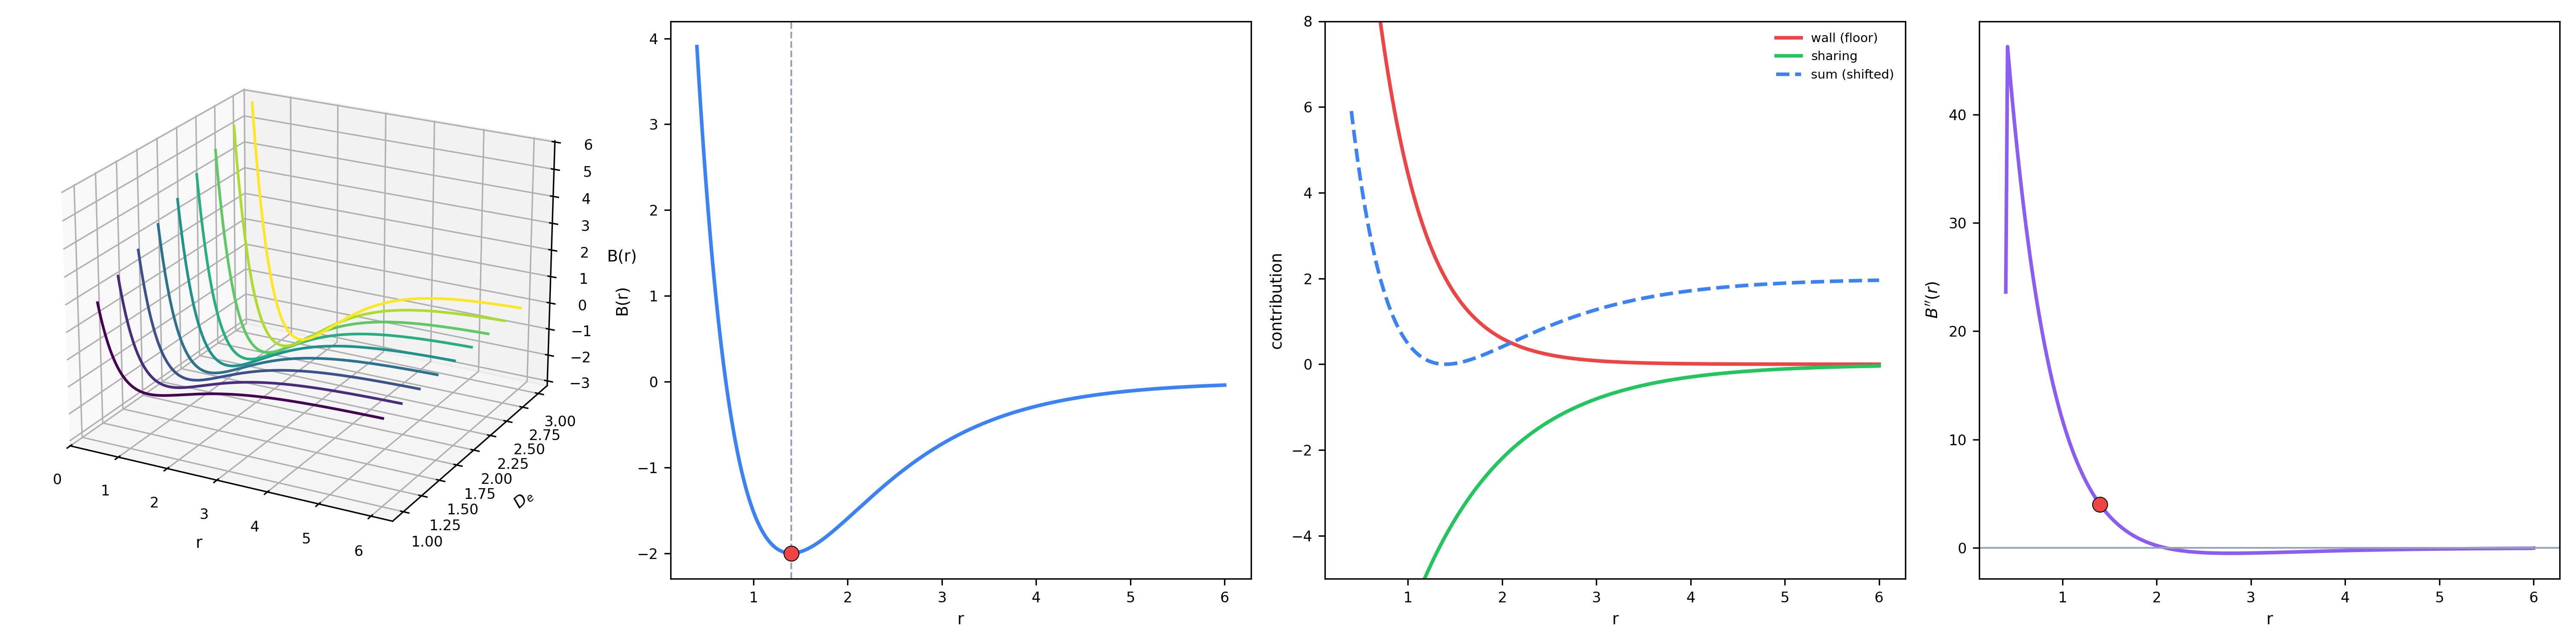
\includegraphics[width=\textwidth]{figures/panel_7_bondlength.png}
    \caption{\textbf{Bond Length as the Convex Thickness Minimiser.}
    (\textbf{A})~Three-dimensional family of joint-thickness wells $B(r)=D_e[(1-e^{-d(r-r_0)})^2-1]$ over internuclear separation $r$ and well depth $D_e$ (viridis), each curve a convex well with a single interior minimum; the minimum deepens with $D_e$ but never moves to $r=0$.
    (\textbf{B})~The thickness profile $B(r)$ (blue) with its unique interior minimiser marked (red point at $r^{*}=1.40$, in units of $r_0$); the dashed line locates $r^{*}$. The curve diverges as $r\to0$ and plateaus as $r\to\infty$, the equilibrium standoff of Theorem~\ref{thm:length}.
    (\textbf{C})~The two competing contributions: the repulsive wall (red, diverging as $r\to0$---the contact floor asserting itself), the sharing pull (green, the boundary-reduction drawing the atoms together), and their sum (blue dashed) with the interior minimum, showing the floor as the origin of short-range repulsion.
    (\textbf{D})~Curvature $B''(r)$ (purple) versus separation; it is positive at the minimiser (red point) and crosses zero only well away from it, confirming the well is locally convex at $r^{*}$ ($B''(r^{*})=3.99>0$).}
    \label{fig:panel_bondlength}
\end{figure*}

% ---------------------------------------------------------------------
\begin{figure*}[!htbp]
    \centering
    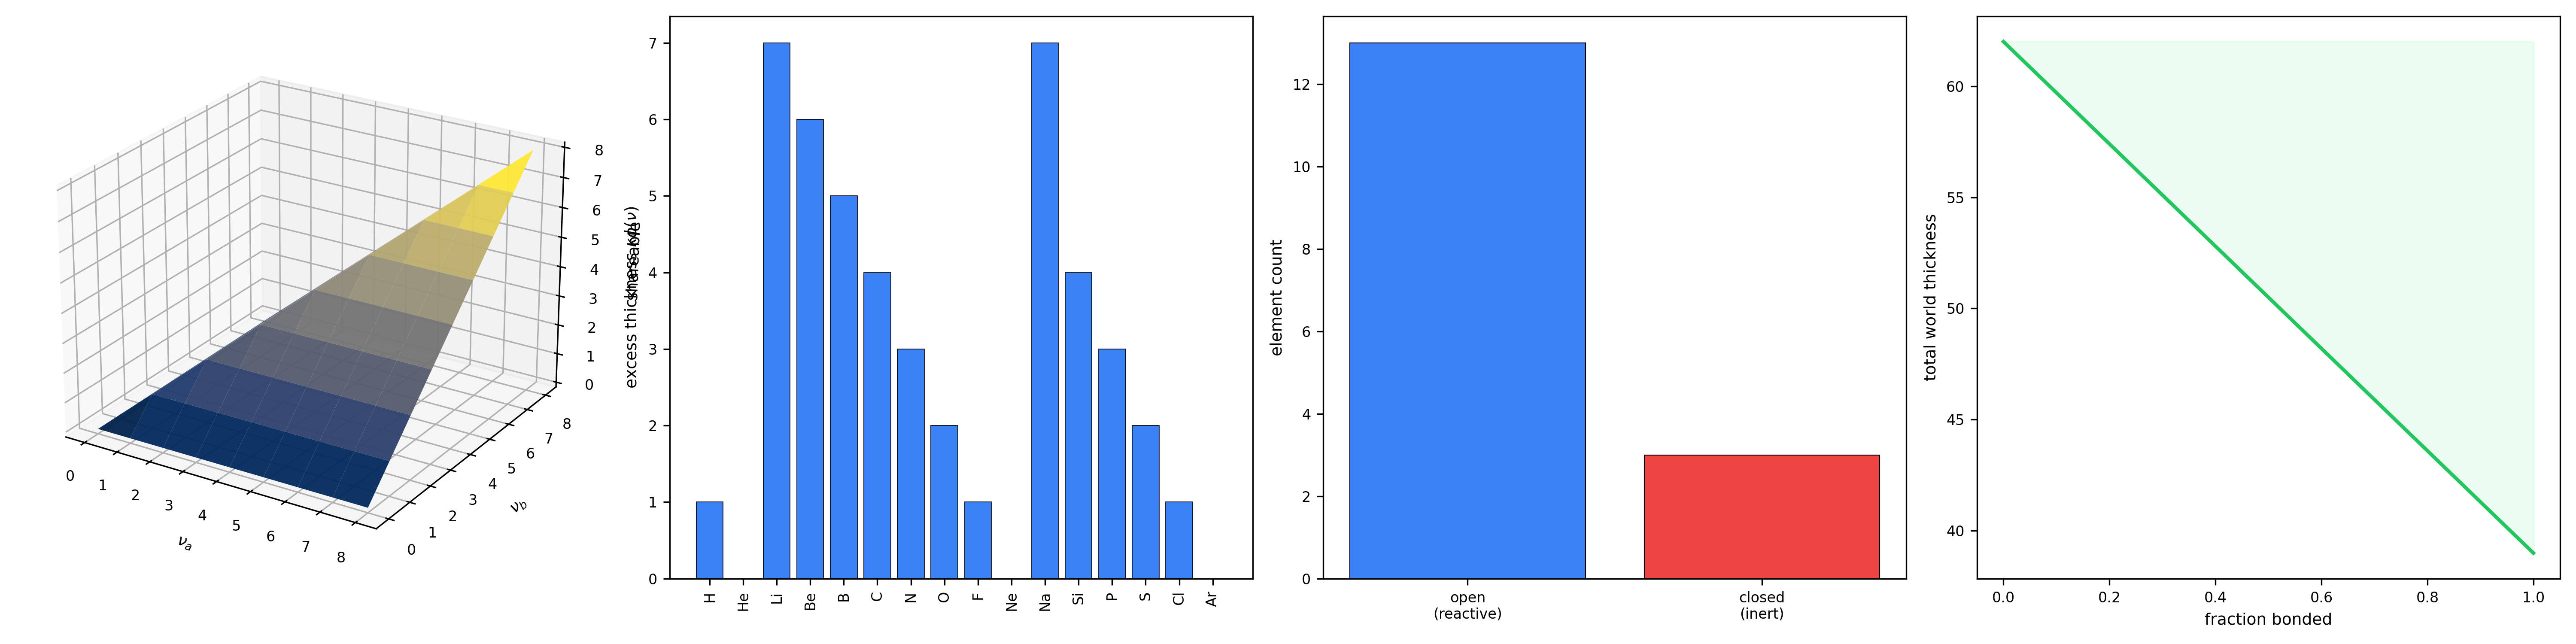
\includegraphics[width=\textwidth]{figures/panel_8_existence.png}
    \caption{\textbf{Why a World of Bounded Atoms Must Be a World of Molecules.}
    (\textbf{A})~Three-dimensional surface of the shareable content $\min(\nu_a,\nu_b)$ over the vacancy plane (cividis): the boundary that two atoms can commit jointly, zero whenever either is closed-shell and rising with the smaller vacancy, the resource from which structure is built.
    (\textbf{B})~Excess boundary thickness $\kappa\phi(\nu)$ above the closed-shell minimum for sixteen elements, bars red where $\nu=0$ (no excess: the noble-gas minimum) and blue where $\nu>0$ (excess to be relaxed by bonding).
    (\textbf{C})~Element census of the open (reactive, blue) versus closed (inert, red) shells among the sixteen elements, the count of atoms that carry shareable vacancy versus those that do not.
    (\textbf{D})~Total world boundary thickness versus the fraction of open atoms that have bonded: the monotone decrease (green, shaded reduction) shows that a world of bounded atoms with positive vacancy lowers its total thickness by forming molecules---chemical structure as the floor's economy (Theorem~\ref{thm:why}).}
    \label{fig:panel_existence}
\end{figure*}
 or copy individually.
% =====================================================================

% ---------------------------------------------------------------------
\begin{figure*}[!htbp]
    \centering
    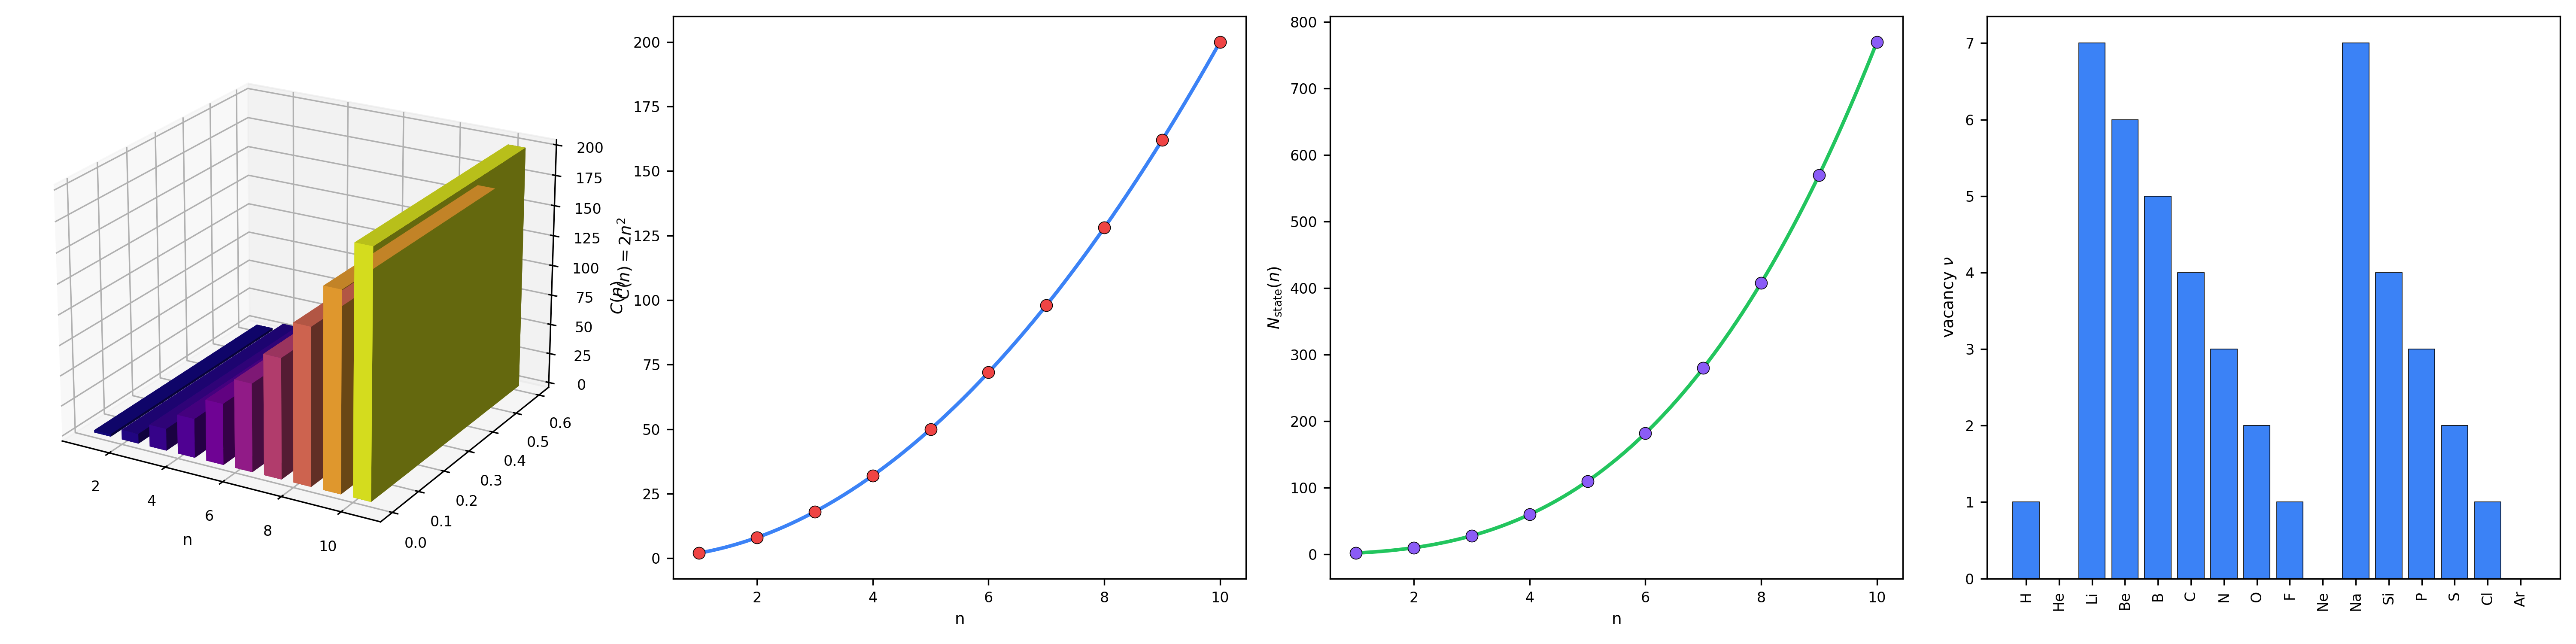
\includegraphics[width=\textwidth]{figures/panel_1_capacity.png}
    \caption{\textbf{Shell Capacity, Cumulative Count, and the Vacancy Ladder.}
    (\textbf{A})~Three-dimensional bar chart of the shell capacity $C(n)=2n^2$ for principal depths $n=1,\ldots,10$, bar height encoding the capacity and colour (plasma scale) tracking its magnitude. The quadratic growth is the derived count $2\sum_{\ell=0}^{n-1}(2\ell+1)=2n^2$ of distinct partition cells at depth $n$, the input the chemical-structure derivation takes from the isolated atom.
    (\textbf{B})~Capacity $C(n)$ on the linear $y$-axis versus depth $n$: the continuous parabola $2n^2$ (blue) with the integer capacities (red points) lying exactly on it for $n=1,\ldots,10$, confirming $C(n)=2n^2$ with no deviation.
    (\textbf{C})~Cumulative partition count $N_{\mathrm{state}}(n)=n(n+1)(2n+1)/3$ (green curve) with the integer cumulative totals (purple points) on the curve, the cubic running sum of the shell capacities.
    (\textbf{D})~Vacancy $\nu=C_v-q_v$ for sixteen elements H through Ar, bars coloured red where $\nu=0$ (closed shell, noble) and blue where $\nu>0$ (open shell). The three red bars are exactly He, Ne, Ar, validating $\nu=0\iff$ noble across all sixteen elements (Theorem~\ref{thm:valence}, Definition~\ref{def:vacancy}).}
    \label{fig:panel_capacity}
\end{figure*}

% ---------------------------------------------------------------------
\begin{figure*}[!htbp]
    \centering
    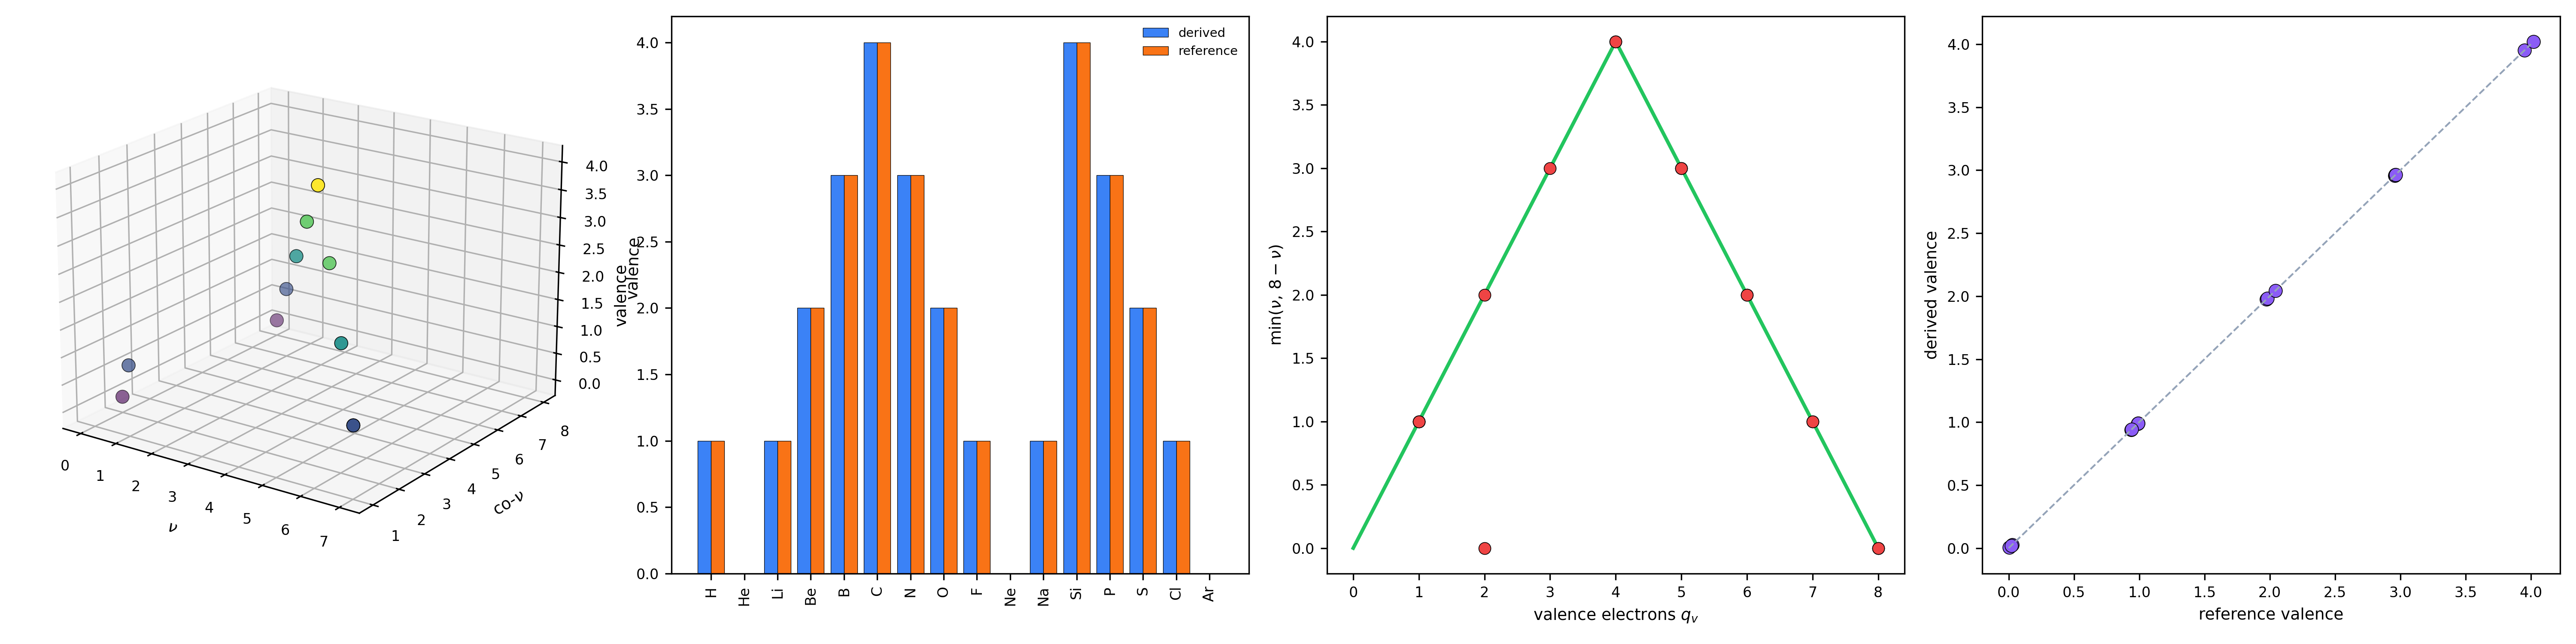
\includegraphics[width=\textwidth]{figures/panel_2_valence.png}
    \caption{\textbf{Valence as the Vacancy Count.}
    (\textbf{A})~Three-dimensional scatter of the sixteen elements in $(\nu,\;C_v-\nu,\;\mathrm{valence})$ space---vacancy against co-vacancy against derived valence---coloured by valence (viridis). The points lie on the surface $\mathrm{valence}=\min(\nu,\,C_v-\nu)$, the covalent-valence rule of Theorem~\ref{thm:valence}.
    (\textbf{B})~Derived valence (blue) and reference common valence (orange) as grouped bars per element. The two series coincide for every element, the $16/16$ agreement of the validation suite.
    (\textbf{C})~The closure curve $\min(\nu,8-\nu)$ (green) over valence-electron count $q_v$, with the elements (red points) sitting on it; the curve peaks at four, recovering carbon's valence of four at $q_v=4$.
    (\textbf{D})~Derived versus reference valence on the identity diagonal (grey dashed); all points lie on the diagonal (small jitter added for visibility), confirming exact reproduction of the common valences from the vacancy arithmetic alone.}
    \label{fig:panel_valence}
\end{figure*}

% ---------------------------------------------------------------------
\begin{figure*}[!htbp]
    \centering
    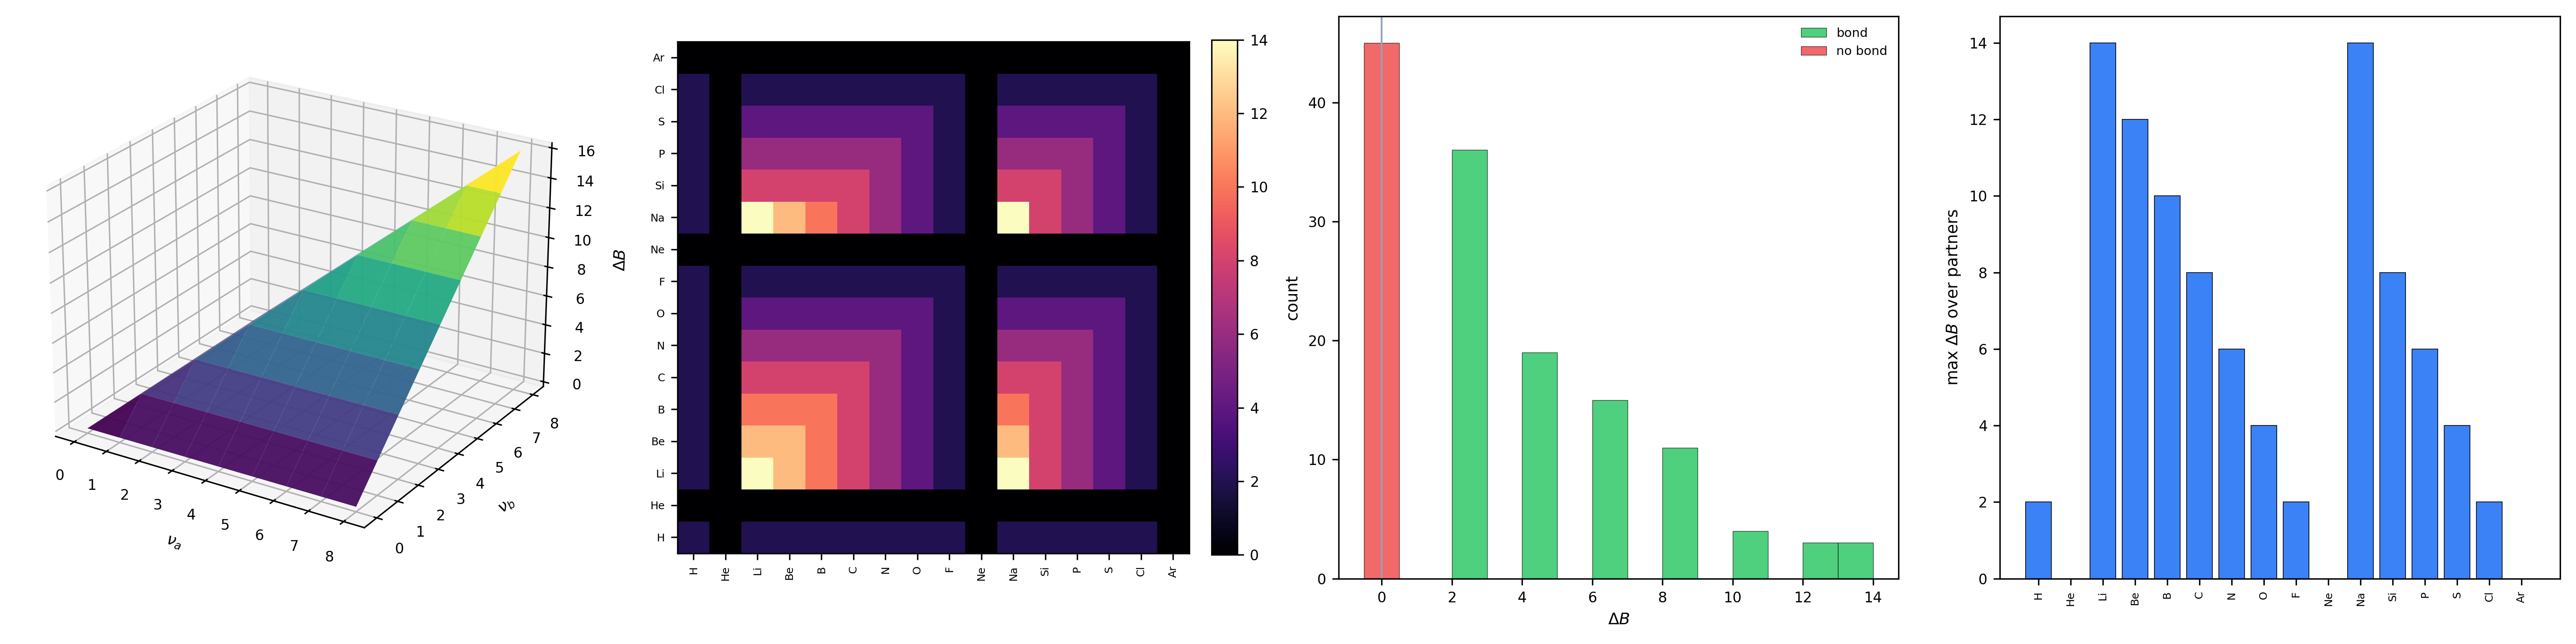
\includegraphics[width=\textwidth]{figures/panel_3_bonding.png}
    \caption{\textbf{The Bonding Criterion over All Element Pairs.}
    (\textbf{A})~Three-dimensional surface of the shared content $\Delta B(\nu_a,\nu_b)$ over the vacancy plane, computed from the monotone thickness model $B=B_0+\kappa\phi(\nu)$ with $\phi(\nu)=\nu$. The surface is positive in the interior and falls to zero along the axes $\nu_a=0$ or $\nu_b=0$: a bond's thickness reduction vanishes whenever either partner is closed-shell (Theorem~\ref{thm:bond}).
    (\textbf{B})~Heatmap of $\Delta B$ across all $136$ element pairs (H through Ar), magma scale. The dark rows and columns are the noble gases He, Ne, Ar, whose shared content is zero with every partner.
    (\textbf{C})~Distribution of $\Delta B$ split into bonding pairs (green, $\Delta B>0$) and non-bonding pairs (red, $\Delta B=0$), separated cleanly about the threshold $\Delta B=0$ (grey line): the sign of $\Delta B$ matches ``neither partner closed-shell'' in all $136$ cases.
    (\textbf{D})~Maximum attainable $\Delta B$ over all partners for each element, bars coloured red for noble (zero) and blue for open-shell. The noble gases alone register zero, the chemical statement that they are inert (Corollary~\ref{cor:noble}).}
    \label{fig:panel_bonding}
\end{figure*}

% ---------------------------------------------------------------------
\begin{figure*}[!htbp]
    \centering
    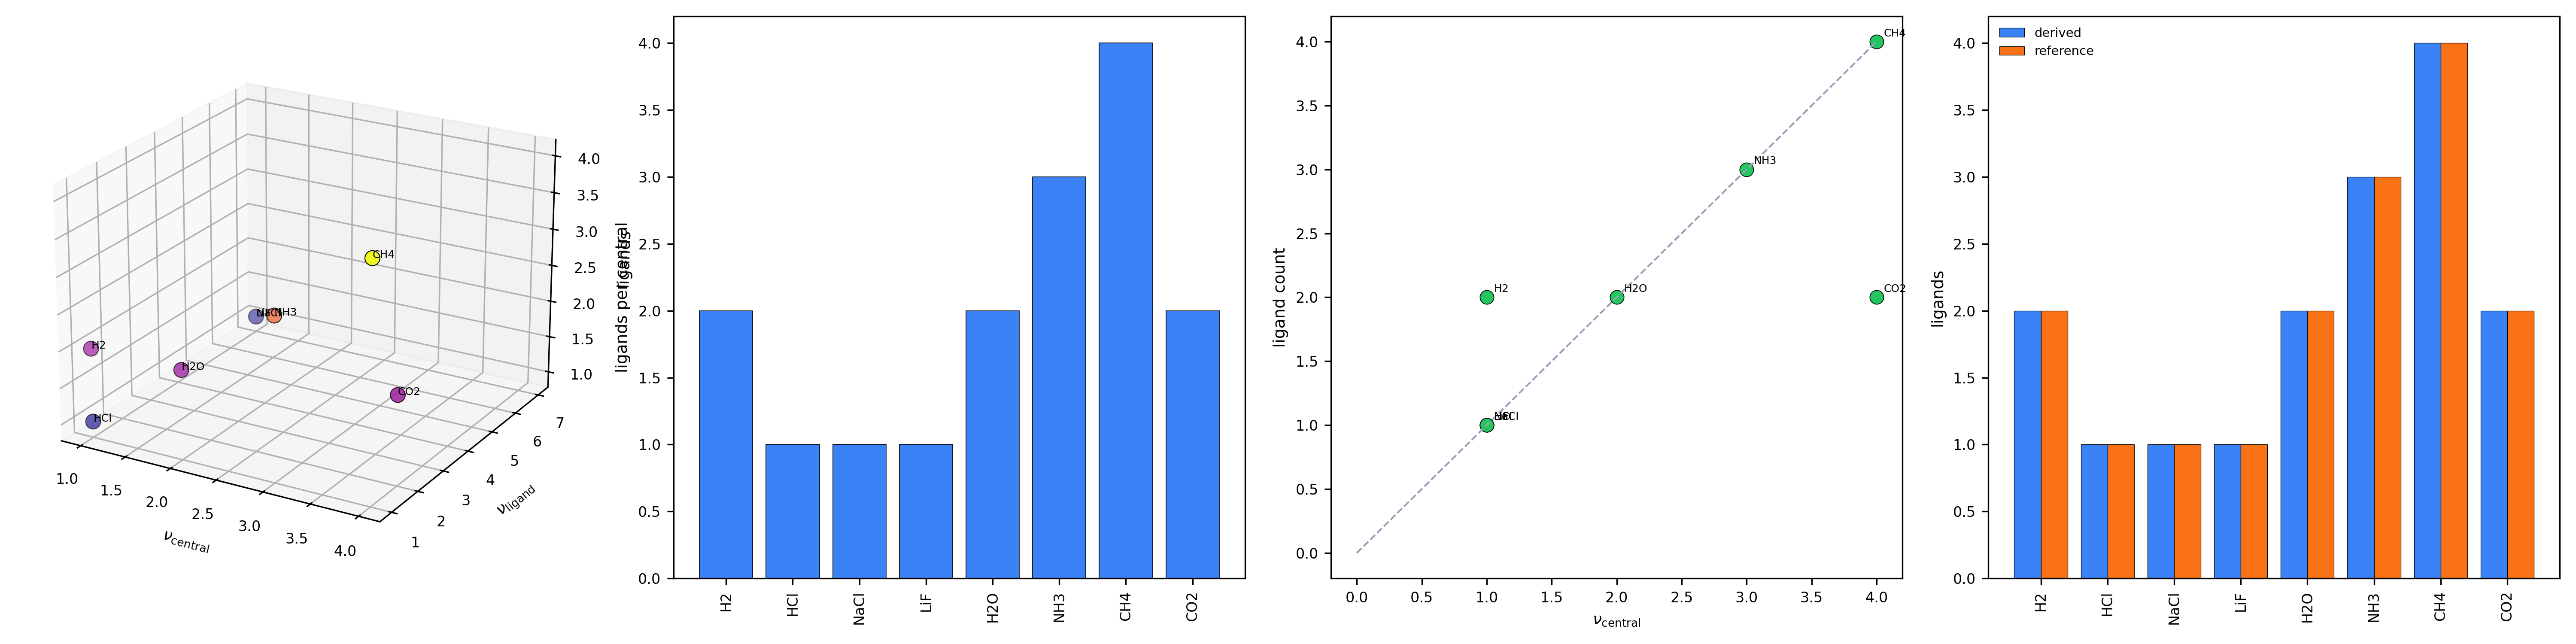
\includegraphics[width=\textwidth]{figures/panel_4_stoichiometry.png}
    \caption{\textbf{Stoichiometry from Vacancy Matching.}
    (\textbf{A})~Three-dimensional scatter of eight molecules in $(\nu_{\mathrm{central}},\,\nu_{\mathrm{ligand}},\,\text{ligand count})$ space, points labelled by molecule and coloured by ligand count (plasma). The ligand count is fixed by closing the central atom's vacancy through interfaces of the ligand's vacancy, recovering the observed formulae.
    (\textbf{B})~Ligands per central atom for H$_2$, HCl, NaCl, LiF, H$_2$O, NH$_3$, CH$_4$, CO$_2$, showing the $1{:}1$, $2{:}1$, $3{:}1$, $4{:}1$ ratios as the central vacancy increases.
    (\textbf{C})~Central vacancy $\nu_{\mathrm{central}}$ versus predicted ligand count; the points track the diagonal (grey dashed) for the hydride series (H$_2$O, NH$_3$, CH$_4$), where each monovalent ligand closes one central vacancy.
    (\textbf{D})~Derived (blue) versus reference (orange) ligand count per molecule as grouped bars; the two coincide for all eight molecules ($8/8$), the vacancy ratio reproducing each stoichiometry with no further input.}
    \label{fig:panel_stoichiometry}
\end{figure*}

% ---------------------------------------------------------------------
\begin{figure*}[!htbp]
    \centering
    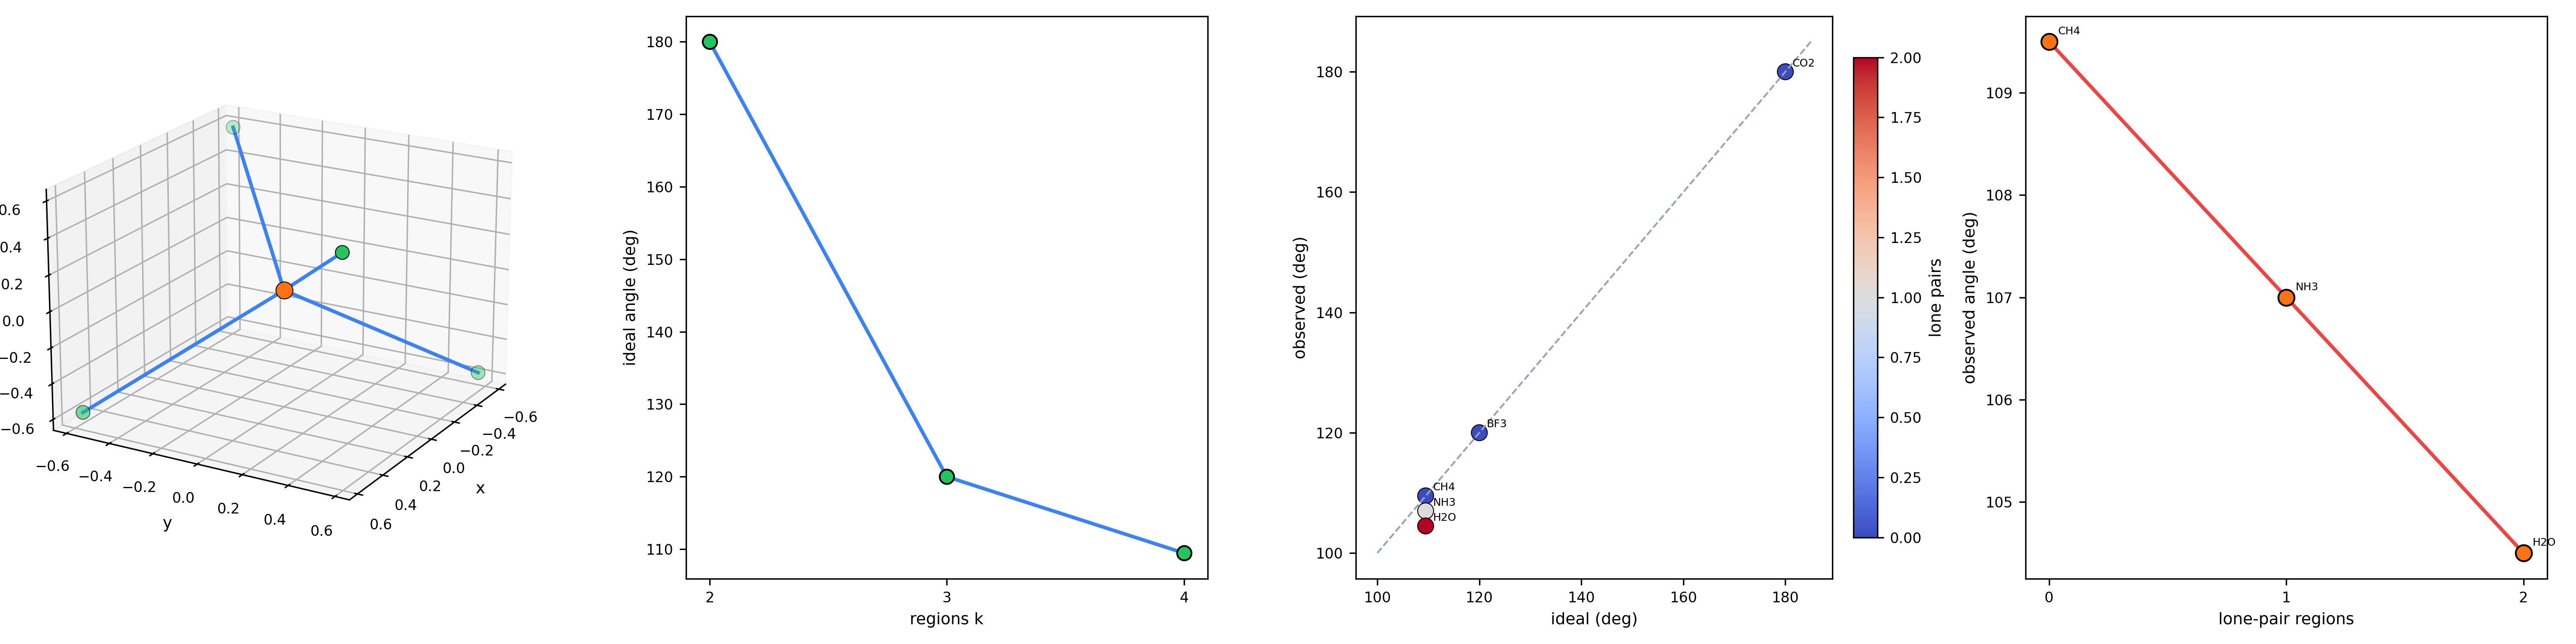
\includegraphics[width=\textwidth]{figures/panel_5_geometry.png}
    \caption{\textbf{Molecular Geometry as Maximal Angular Separation.}
    (\textbf{A})~Three-dimensional rendering of the four maximally separated bond directions of a four-coordinate centre (methane): bonds (blue) from the central atom (orange) to the four ligand directions (green) at the regular-tetrahedron vertices, the configuration that minimises pairwise solid-angle overlap (Theorem~\ref{thm:geometry}).
    (\textbf{B})~Ideal symmetric bond angle versus number of interface regions $k$: $180^\circ$ ($k=2$, linear), $120^\circ$ ($k=3$, trigonal planar), $109.47^\circ$ ($k=4$, tetrahedral)---the maximal-separation angles of $k$ points on the sphere.
    (\textbf{C})~Observed versus ideal symmetric angle for five molecules, coloured by lone-pair count (coolwarm); points on the diagonal (grey dashed) are the lone-pair-free backbones (CO$_2$, BF$_3$, CH$_4$), and points below it are the lone-pair-compressed geometries (NH$_3$, H$_2$O).
    (\textbf{D})~Observed angle of the four-region family versus lone-pair count: $109.5^\circ$ (CH$_4$, none) $\to 107^\circ$ (NH$_3$, one) $\to 104.5^\circ$ (H$_2$O, two), the monotone compression as unshared regions are added.}
    \label{fig:panel_geometry}
\end{figure*}

% ---------------------------------------------------------------------
\begin{figure*}[!htbp]
    \centering
    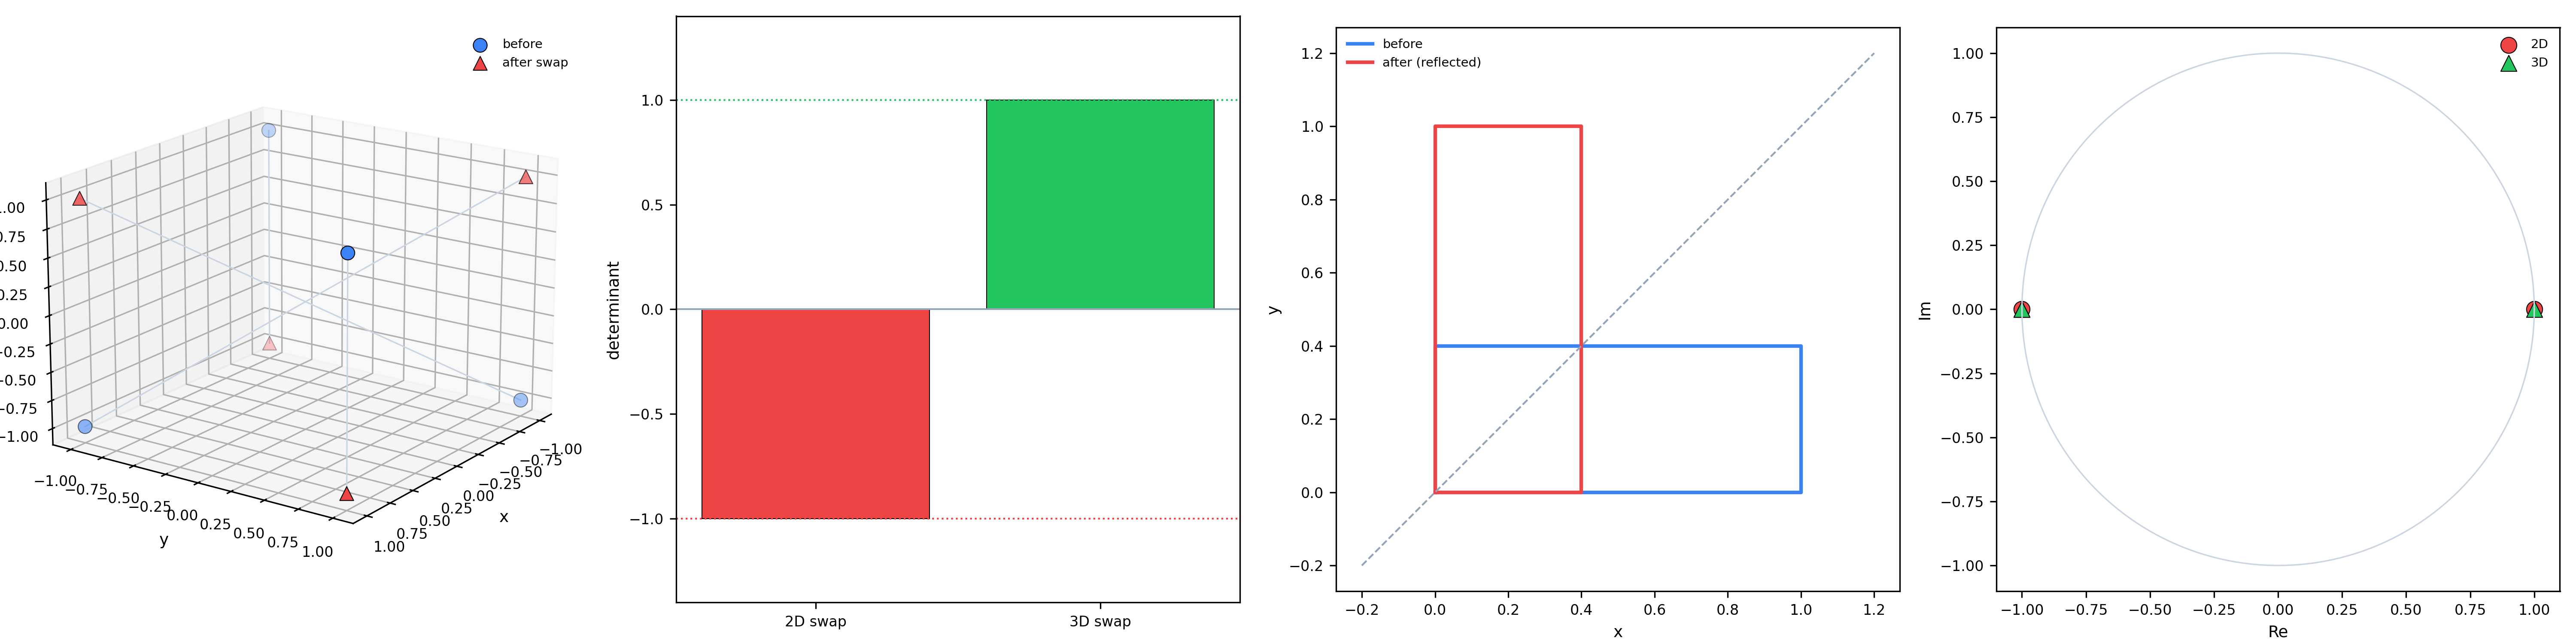
\includegraphics[width=\textwidth]{figures/panel_6_dimension.png}
    \caption{\textbf{Three Dimensions and the Absence of a Privileged Axis.}
    (\textbf{A})~Three-dimensional action of the axis-swap $(x,y,z)\mapsto(y,x,-z)$ on the vertices of a tetrahedron: original vertices (blue) and their images (red triangles) joined by displacement lines. The swap is realised as a continuous proper rotation, exchanging the two axes by an internal motion (Principle~\ref{prin:threed}).
    (\textbf{B})~Determinants of the axis-swap matrices: the two-dimensional swap has determinant $-1$ (a reflection, red) and the three-dimensional swap has determinant $+1$ (a proper rotation in $SO(3)$, green), the dashed guides marking $\pm1$.
    (\textbf{C})~The two-dimensional swap as a reflection across the line $y=x$ (grey dashed): a rectangle (blue) mapped to its mirror image (red), showing that in $d=2$ exchanging the axes requires a reflection, not an internal rotation---hence an external choice.
    (\textbf{D})~Eigenvalue spectra of the two swap matrices on the unit circle (grey): the two-dimensional swap (red) has eigenvalues $\pm1$, the three-dimensional swap (green triangles) has eigenvalues consistent with a proper rotation, confirming $d=3$ as the minimum dimension of selector-free axis exchange.}
    \label{fig:panel_dimension}
\end{figure*}

% ---------------------------------------------------------------------
\begin{figure*}[!htbp]
    \centering
    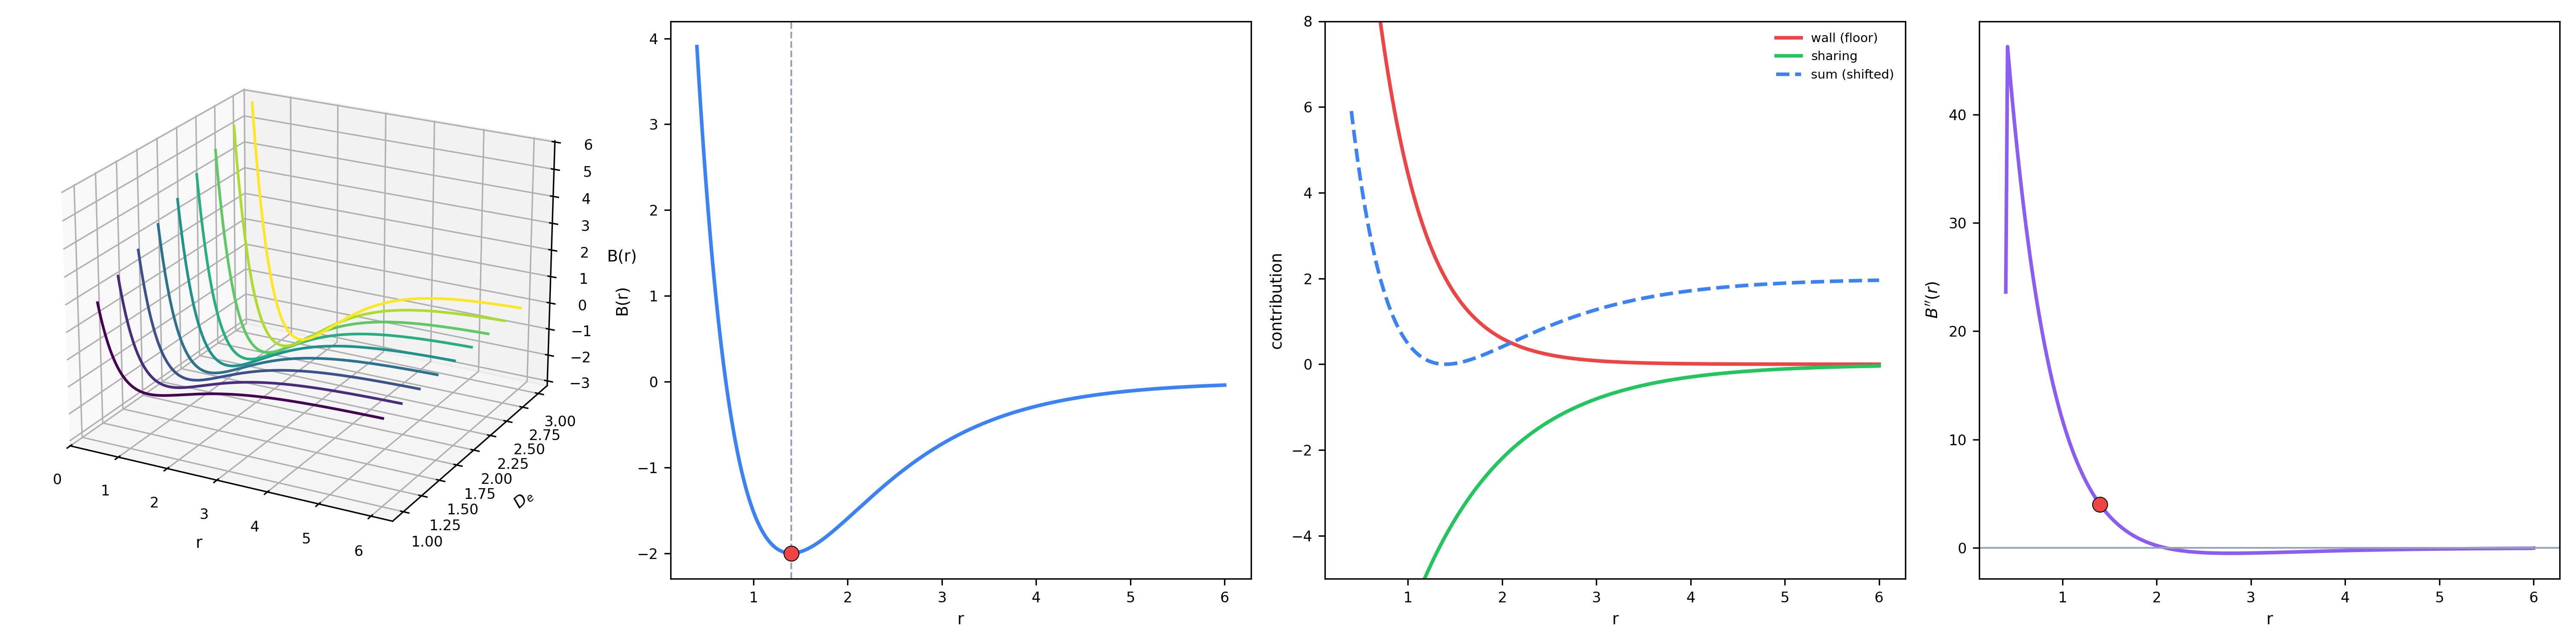
\includegraphics[width=\textwidth]{figures/panel_7_bondlength.png}
    \caption{\textbf{Bond Length as the Convex Thickness Minimiser.}
    (\textbf{A})~Three-dimensional family of joint-thickness wells $B(r)=D_e[(1-e^{-d(r-r_0)})^2-1]$ over internuclear separation $r$ and well depth $D_e$ (viridis), each curve a convex well with a single interior minimum; the minimum deepens with $D_e$ but never moves to $r=0$.
    (\textbf{B})~The thickness profile $B(r)$ (blue) with its unique interior minimiser marked (red point at $r^{*}=1.40$, in units of $r_0$); the dashed line locates $r^{*}$. The curve diverges as $r\to0$ and plateaus as $r\to\infty$, the equilibrium standoff of Theorem~\ref{thm:length}.
    (\textbf{C})~The two competing contributions: the repulsive wall (red, diverging as $r\to0$---the contact floor asserting itself), the sharing pull (green, the boundary-reduction drawing the atoms together), and their sum (blue dashed) with the interior minimum, showing the floor as the origin of short-range repulsion.
    (\textbf{D})~Curvature $B''(r)$ (purple) versus separation; it is positive at the minimiser (red point) and crosses zero only well away from it, confirming the well is locally convex at $r^{*}$ ($B''(r^{*})=3.99>0$).}
    \label{fig:panel_bondlength}
\end{figure*}

% ---------------------------------------------------------------------
\begin{figure*}[!htbp]
    \centering
    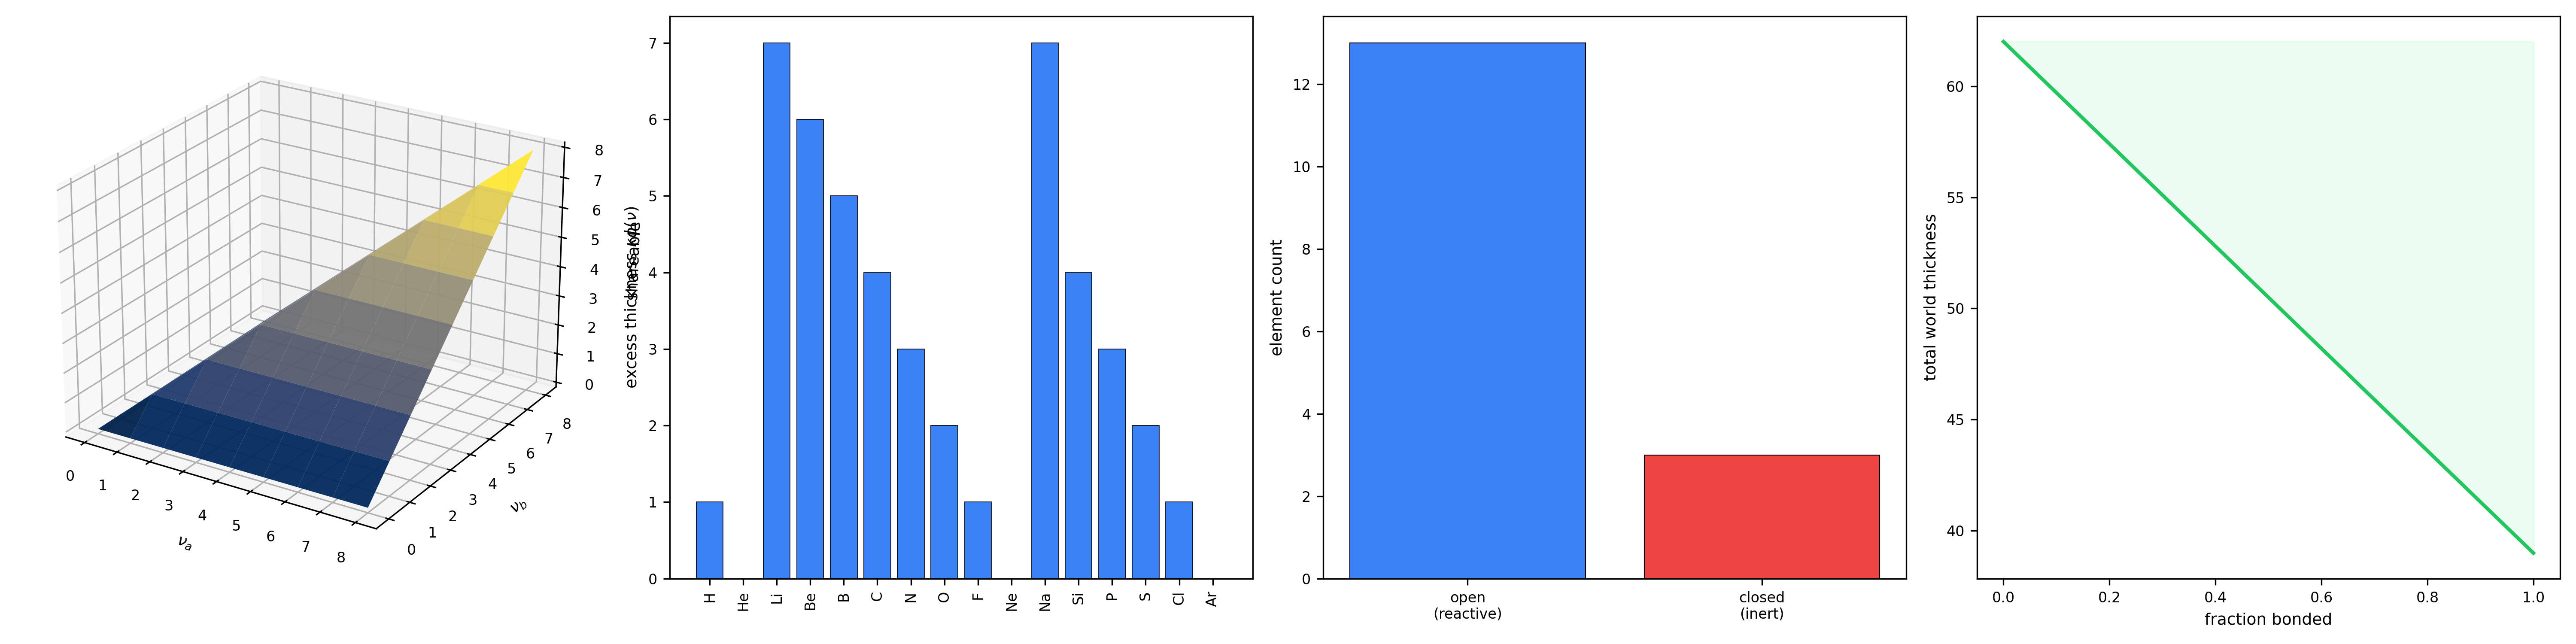
\includegraphics[width=\textwidth]{figures/panel_8_existence.png}
    \caption{\textbf{Why a World of Bounded Atoms Must Be a World of Molecules.}
    (\textbf{A})~Three-dimensional surface of the shareable content $\min(\nu_a,\nu_b)$ over the vacancy plane (cividis): the boundary that two atoms can commit jointly, zero whenever either is closed-shell and rising with the smaller vacancy, the resource from which structure is built.
    (\textbf{B})~Excess boundary thickness $\kappa\phi(\nu)$ above the closed-shell minimum for sixteen elements, bars red where $\nu=0$ (no excess: the noble-gas minimum) and blue where $\nu>0$ (excess to be relaxed by bonding).
    (\textbf{C})~Element census of the open (reactive, blue) versus closed (inert, red) shells among the sixteen elements, the count of atoms that carry shareable vacancy versus those that do not.
    (\textbf{D})~Total world boundary thickness versus the fraction of open atoms that have bonded: the monotone decrease (green, shaded reduction) shows that a world of bounded atoms with positive vacancy lowers its total thickness by forming molecules---chemical structure as the floor's economy (Theorem~\ref{thm:why}).}
    \label{fig:panel_existence}
\end{figure*}
 or copy individually.
% =====================================================================

% ---------------------------------------------------------------------
\begin{figure*}[!htbp]
    \centering
    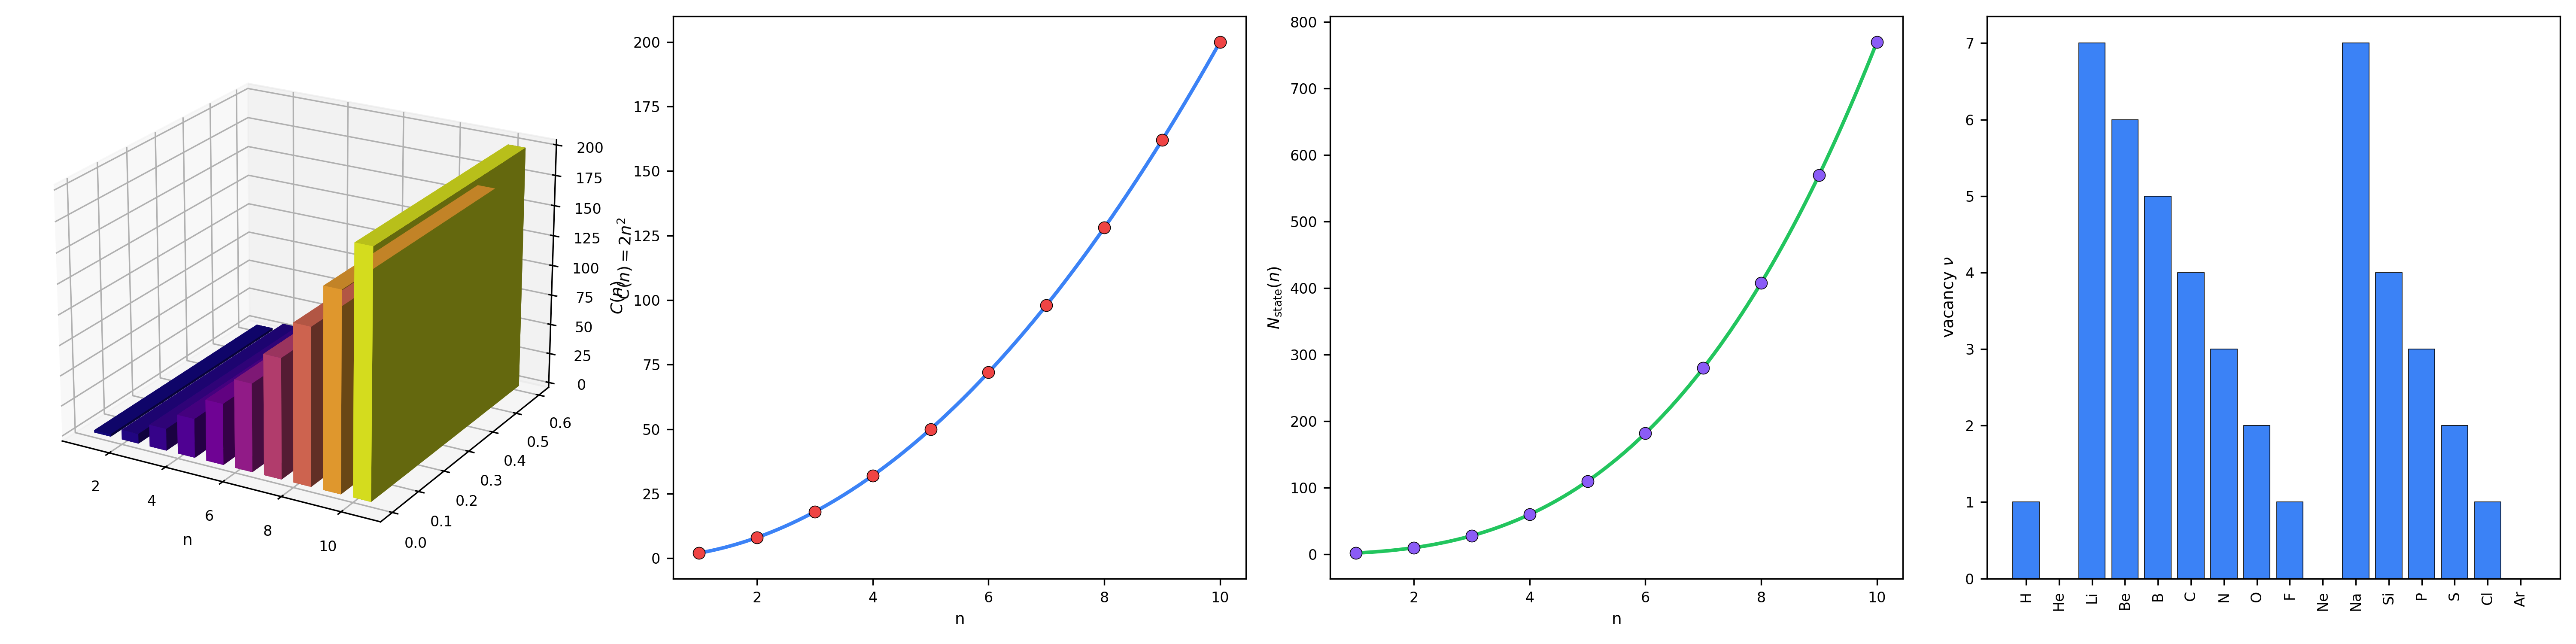
\includegraphics[width=\textwidth]{figures/panel_1_capacity.png}
    \caption{\textbf{Shell Capacity, Cumulative Count, and the Vacancy Ladder.}
    (\textbf{A})~Three-dimensional bar chart of the shell capacity $C(n)=2n^2$ for principal depths $n=1,\ldots,10$, bar height encoding the capacity and colour (plasma scale) tracking its magnitude. The quadratic growth is the derived count $2\sum_{\ell=0}^{n-1}(2\ell+1)=2n^2$ of distinct partition cells at depth $n$, the input the chemical-structure derivation takes from the isolated atom.
    (\textbf{B})~Capacity $C(n)$ on the linear $y$-axis versus depth $n$: the continuous parabola $2n^2$ (blue) with the integer capacities (red points) lying exactly on it for $n=1,\ldots,10$, confirming $C(n)=2n^2$ with no deviation.
    (\textbf{C})~Cumulative partition count $N_{\mathrm{state}}(n)=n(n+1)(2n+1)/3$ (green curve) with the integer cumulative totals (purple points) on the curve, the cubic running sum of the shell capacities.
    (\textbf{D})~Vacancy $\nu=C_v-q_v$ for sixteen elements H through Ar, bars coloured red where $\nu=0$ (closed shell, noble) and blue where $\nu>0$ (open shell). The three red bars are exactly He, Ne, Ar, validating $\nu=0\iff$ noble across all sixteen elements (Theorem~\ref{thm:valence}, Definition~\ref{def:vacancy}).}
    \label{fig:panel_capacity}
\end{figure*}

% ---------------------------------------------------------------------
\begin{figure*}[!htbp]
    \centering
    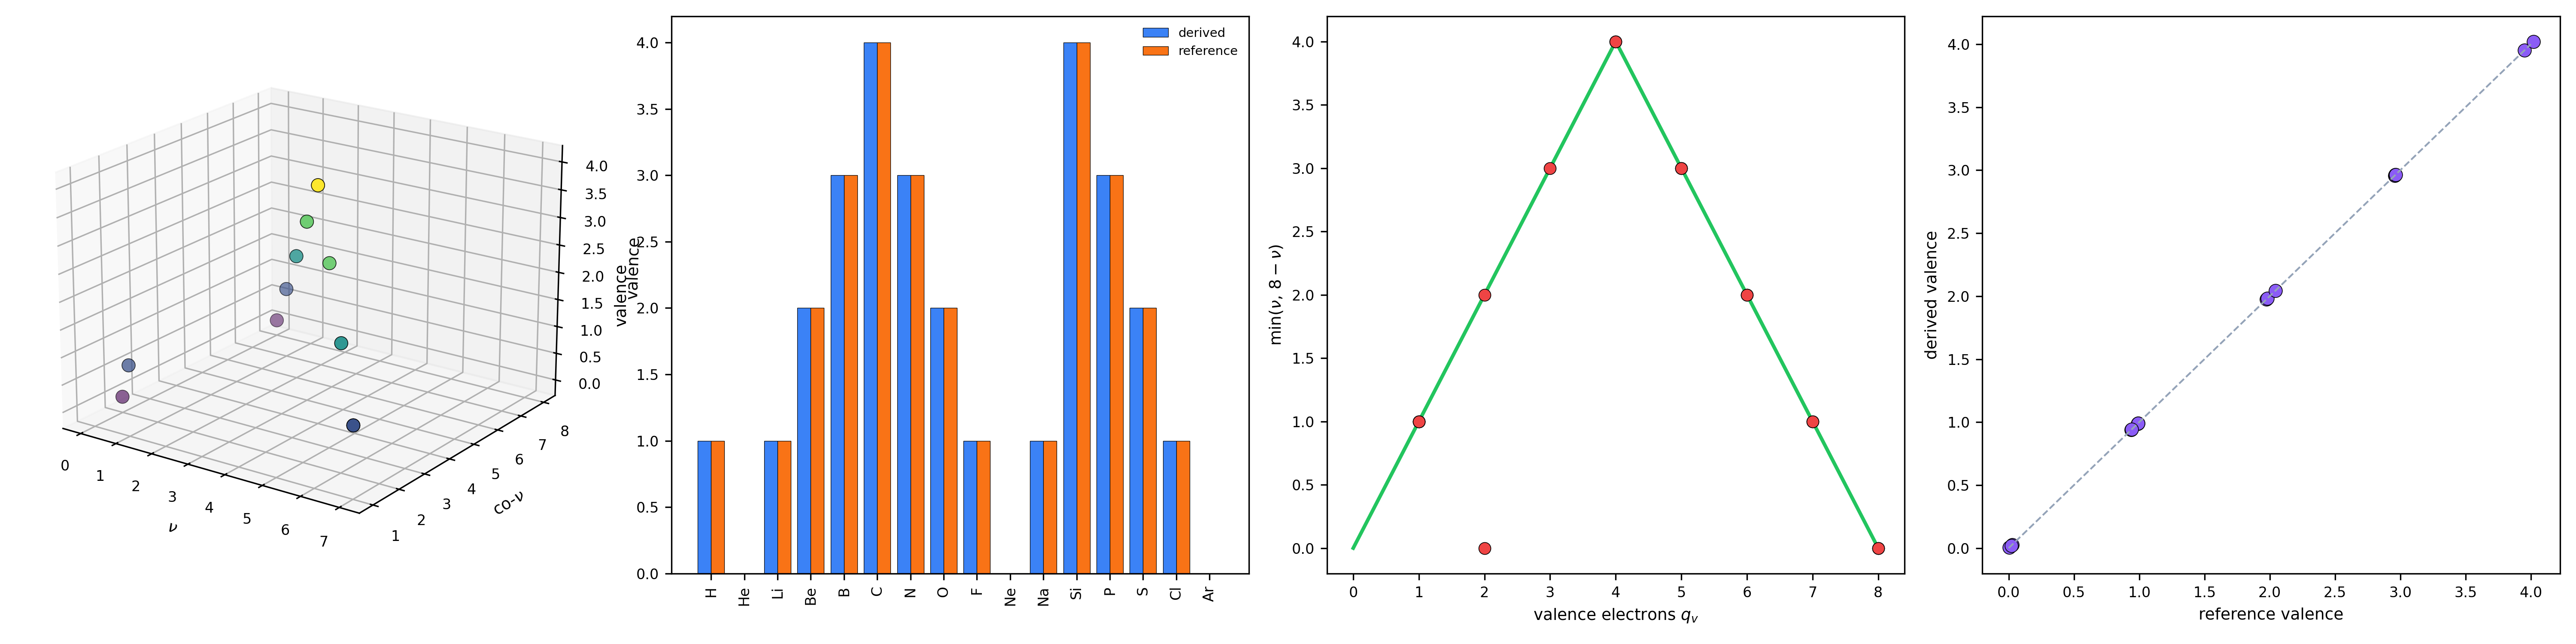
\includegraphics[width=\textwidth]{figures/panel_2_valence.png}
    \caption{\textbf{Valence as the Vacancy Count.}
    (\textbf{A})~Three-dimensional scatter of the sixteen elements in $(\nu,\;C_v-\nu,\;\mathrm{valence})$ space---vacancy against co-vacancy against derived valence---coloured by valence (viridis). The points lie on the surface $\mathrm{valence}=\min(\nu,\,C_v-\nu)$, the covalent-valence rule of Theorem~\ref{thm:valence}.
    (\textbf{B})~Derived valence (blue) and reference common valence (orange) as grouped bars per element. The two series coincide for every element, the $16/16$ agreement of the validation suite.
    (\textbf{C})~The closure curve $\min(\nu,8-\nu)$ (green) over valence-electron count $q_v$, with the elements (red points) sitting on it; the curve peaks at four, recovering carbon's valence of four at $q_v=4$.
    (\textbf{D})~Derived versus reference valence on the identity diagonal (grey dashed); all points lie on the diagonal (small jitter added for visibility), confirming exact reproduction of the common valences from the vacancy arithmetic alone.}
    \label{fig:panel_valence}
\end{figure*}

% ---------------------------------------------------------------------
\begin{figure*}[!htbp]
    \centering
    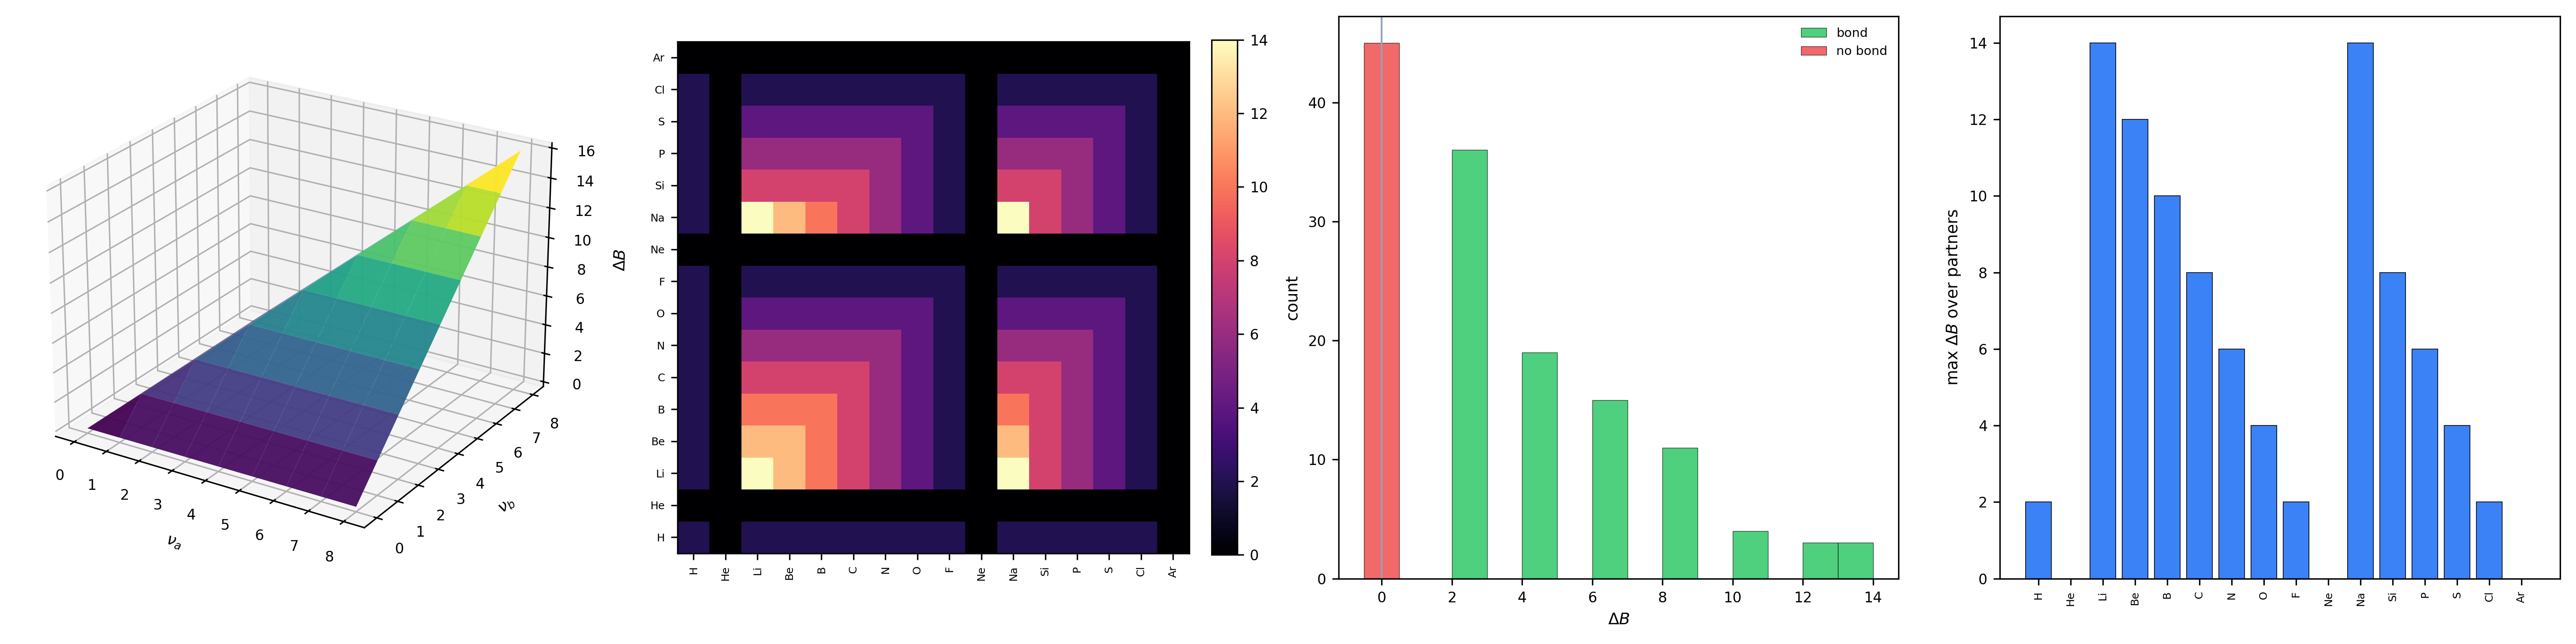
\includegraphics[width=\textwidth]{figures/panel_3_bonding.png}
    \caption{\textbf{The Bonding Criterion over All Element Pairs.}
    (\textbf{A})~Three-dimensional surface of the shared content $\Delta B(\nu_a,\nu_b)$ over the vacancy plane, computed from the monotone thickness model $B=B_0+\kappa\phi(\nu)$ with $\phi(\nu)=\nu$. The surface is positive in the interior and falls to zero along the axes $\nu_a=0$ or $\nu_b=0$: a bond's thickness reduction vanishes whenever either partner is closed-shell (Theorem~\ref{thm:bond}).
    (\textbf{B})~Heatmap of $\Delta B$ across all $136$ element pairs (H through Ar), magma scale. The dark rows and columns are the noble gases He, Ne, Ar, whose shared content is zero with every partner.
    (\textbf{C})~Distribution of $\Delta B$ split into bonding pairs (green, $\Delta B>0$) and non-bonding pairs (red, $\Delta B=0$), separated cleanly about the threshold $\Delta B=0$ (grey line): the sign of $\Delta B$ matches ``neither partner closed-shell'' in all $136$ cases.
    (\textbf{D})~Maximum attainable $\Delta B$ over all partners for each element, bars coloured red for noble (zero) and blue for open-shell. The noble gases alone register zero, the chemical statement that they are inert (Corollary~\ref{cor:noble}).}
    \label{fig:panel_bonding}
\end{figure*}

% ---------------------------------------------------------------------
\begin{figure*}[!htbp]
    \centering
    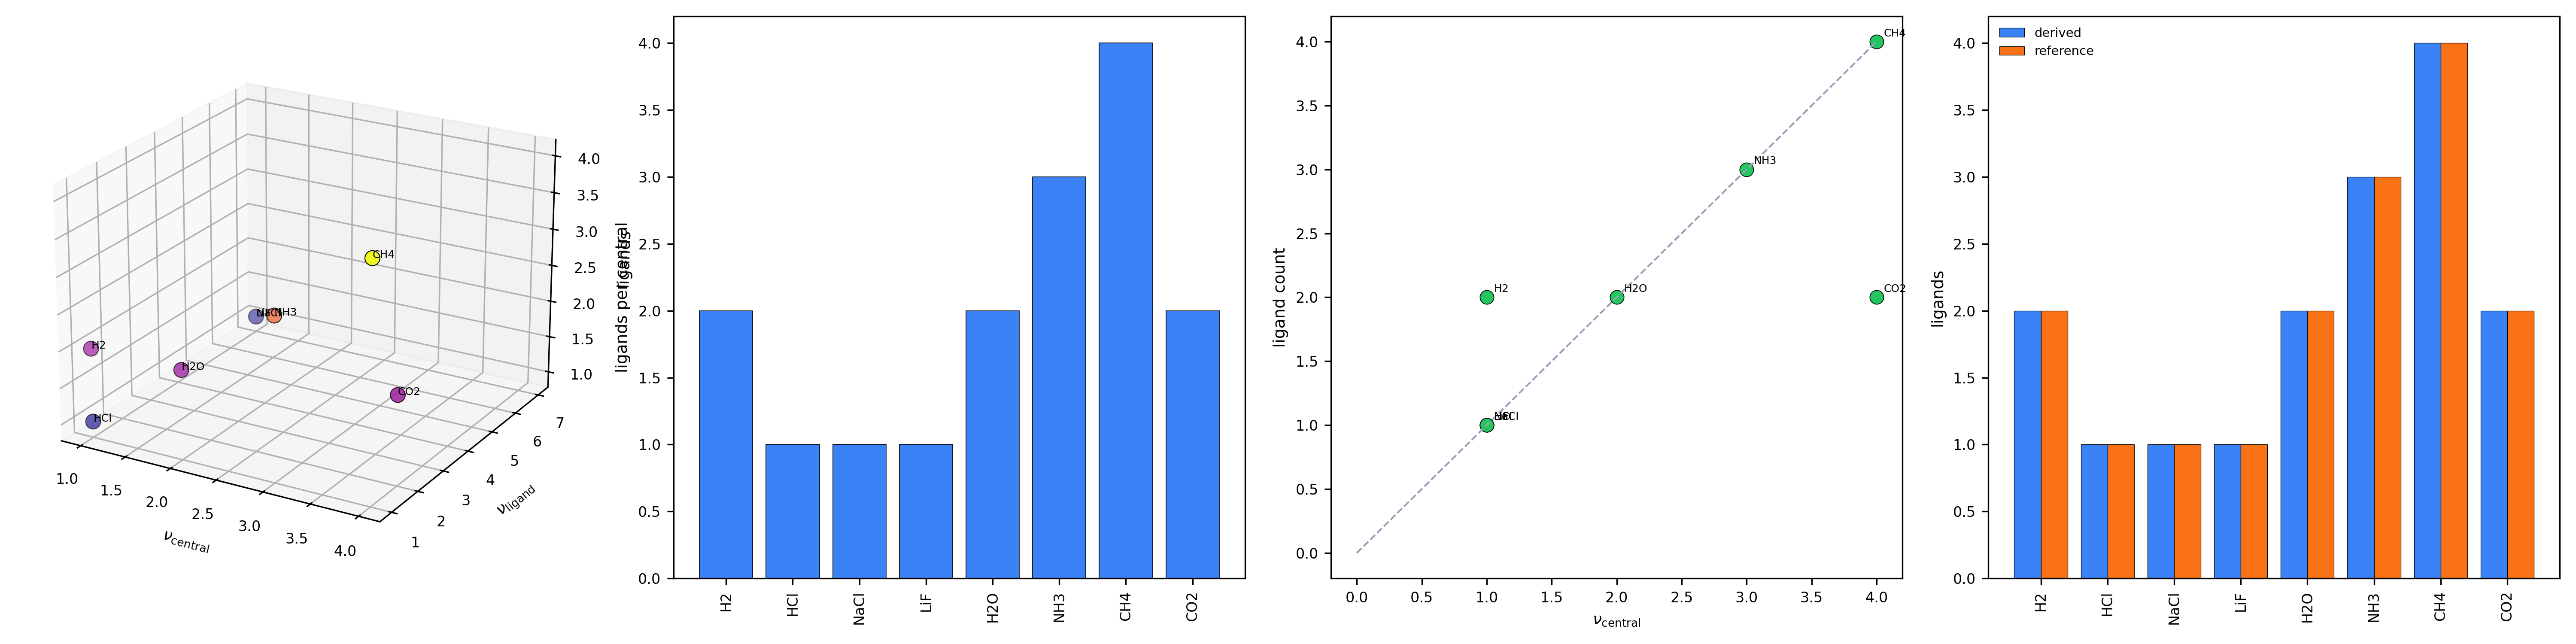
\includegraphics[width=\textwidth]{figures/panel_4_stoichiometry.png}
    \caption{\textbf{Stoichiometry from Vacancy Matching.}
    (\textbf{A})~Three-dimensional scatter of eight molecules in $(\nu_{\mathrm{central}},\,\nu_{\mathrm{ligand}},\,\text{ligand count})$ space, points labelled by molecule and coloured by ligand count (plasma). The ligand count is fixed by closing the central atom's vacancy through interfaces of the ligand's vacancy, recovering the observed formulae.
    (\textbf{B})~Ligands per central atom for H$_2$, HCl, NaCl, LiF, H$_2$O, NH$_3$, CH$_4$, CO$_2$, showing the $1{:}1$, $2{:}1$, $3{:}1$, $4{:}1$ ratios as the central vacancy increases.
    (\textbf{C})~Central vacancy $\nu_{\mathrm{central}}$ versus predicted ligand count; the points track the diagonal (grey dashed) for the hydride series (H$_2$O, NH$_3$, CH$_4$), where each monovalent ligand closes one central vacancy.
    (\textbf{D})~Derived (blue) versus reference (orange) ligand count per molecule as grouped bars; the two coincide for all eight molecules ($8/8$), the vacancy ratio reproducing each stoichiometry with no further input.}
    \label{fig:panel_stoichiometry}
\end{figure*}

% ---------------------------------------------------------------------
\begin{figure*}[!htbp]
    \centering
    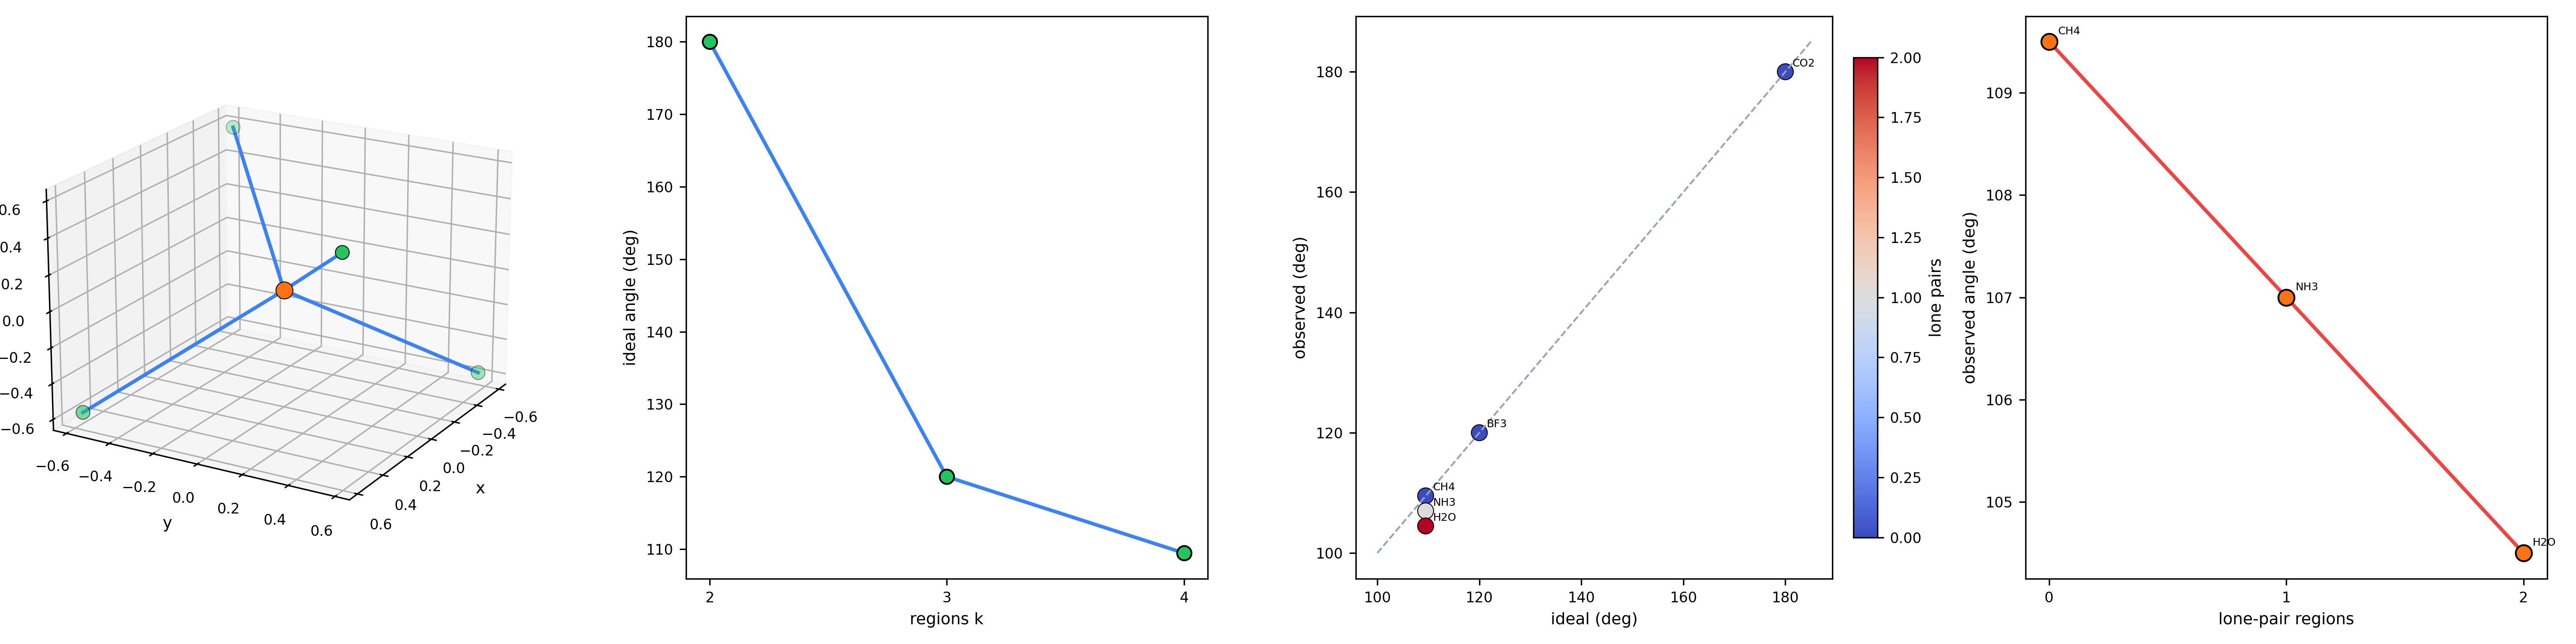
\includegraphics[width=\textwidth]{figures/panel_5_geometry.png}
    \caption{\textbf{Molecular Geometry as Maximal Angular Separation.}
    (\textbf{A})~Three-dimensional rendering of the four maximally separated bond directions of a four-coordinate centre (methane): bonds (blue) from the central atom (orange) to the four ligand directions (green) at the regular-tetrahedron vertices, the configuration that minimises pairwise solid-angle overlap (Theorem~\ref{thm:geometry}).
    (\textbf{B})~Ideal symmetric bond angle versus number of interface regions $k$: $180^\circ$ ($k=2$, linear), $120^\circ$ ($k=3$, trigonal planar), $109.47^\circ$ ($k=4$, tetrahedral)---the maximal-separation angles of $k$ points on the sphere.
    (\textbf{C})~Observed versus ideal symmetric angle for five molecules, coloured by lone-pair count (coolwarm); points on the diagonal (grey dashed) are the lone-pair-free backbones (CO$_2$, BF$_3$, CH$_4$), and points below it are the lone-pair-compressed geometries (NH$_3$, H$_2$O).
    (\textbf{D})~Observed angle of the four-region family versus lone-pair count: $109.5^\circ$ (CH$_4$, none) $\to 107^\circ$ (NH$_3$, one) $\to 104.5^\circ$ (H$_2$O, two), the monotone compression as unshared regions are added.}
    \label{fig:panel_geometry}
\end{figure*}

% ---------------------------------------------------------------------
\begin{figure*}[!htbp]
    \centering
    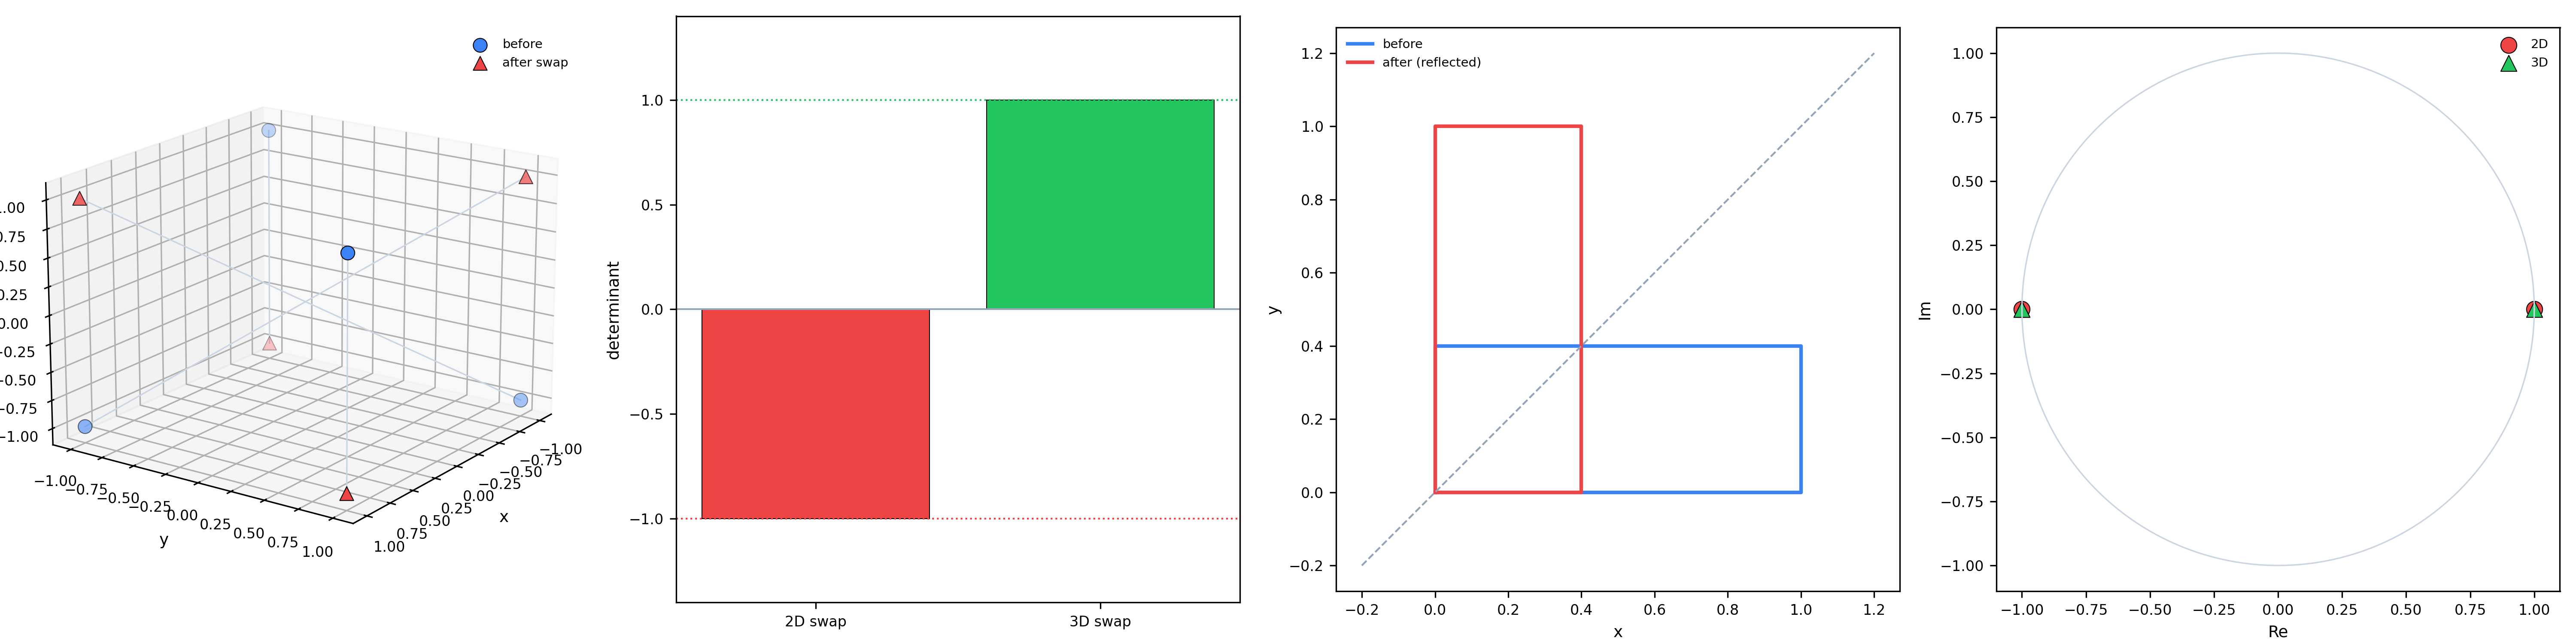
\includegraphics[width=\textwidth]{figures/panel_6_dimension.png}
    \caption{\textbf{Three Dimensions and the Absence of a Privileged Axis.}
    (\textbf{A})~Three-dimensional action of the axis-swap $(x,y,z)\mapsto(y,x,-z)$ on the vertices of a tetrahedron: original vertices (blue) and their images (red triangles) joined by displacement lines. The swap is realised as a continuous proper rotation, exchanging the two axes by an internal motion (Principle~\ref{prin:threed}).
    (\textbf{B})~Determinants of the axis-swap matrices: the two-dimensional swap has determinant $-1$ (a reflection, red) and the three-dimensional swap has determinant $+1$ (a proper rotation in $SO(3)$, green), the dashed guides marking $\pm1$.
    (\textbf{C})~The two-dimensional swap as a reflection across the line $y=x$ (grey dashed): a rectangle (blue) mapped to its mirror image (red), showing that in $d=2$ exchanging the axes requires a reflection, not an internal rotation---hence an external choice.
    (\textbf{D})~Eigenvalue spectra of the two swap matrices on the unit circle (grey): the two-dimensional swap (red) has eigenvalues $\pm1$, the three-dimensional swap (green triangles) has eigenvalues consistent with a proper rotation, confirming $d=3$ as the minimum dimension of selector-free axis exchange.}
    \label{fig:panel_dimension}
\end{figure*}

% ---------------------------------------------------------------------
\begin{figure*}[!htbp]
    \centering
    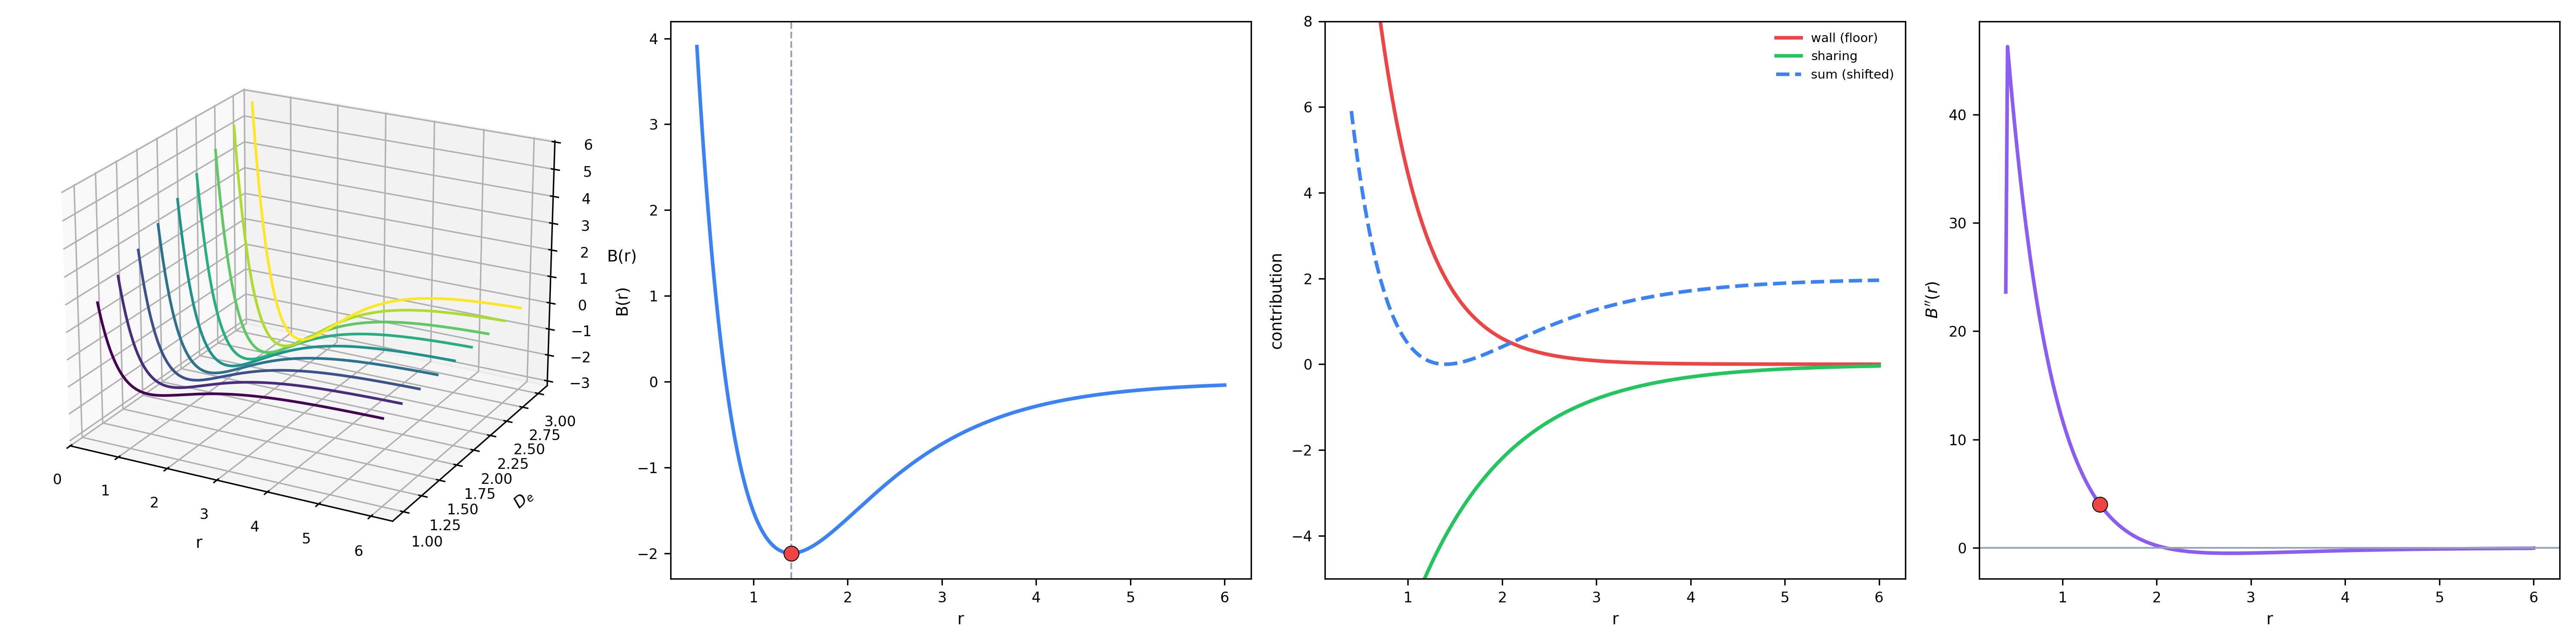
\includegraphics[width=\textwidth]{figures/panel_7_bondlength.png}
    \caption{\textbf{Bond Length as the Convex Thickness Minimiser.}
    (\textbf{A})~Three-dimensional family of joint-thickness wells $B(r)=D_e[(1-e^{-d(r-r_0)})^2-1]$ over internuclear separation $r$ and well depth $D_e$ (viridis), each curve a convex well with a single interior minimum; the minimum deepens with $D_e$ but never moves to $r=0$.
    (\textbf{B})~The thickness profile $B(r)$ (blue) with its unique interior minimiser marked (red point at $r^{*}=1.40$, in units of $r_0$); the dashed line locates $r^{*}$. The curve diverges as $r\to0$ and plateaus as $r\to\infty$, the equilibrium standoff of Theorem~\ref{thm:length}.
    (\textbf{C})~The two competing contributions: the repulsive wall (red, diverging as $r\to0$---the contact floor asserting itself), the sharing pull (green, the boundary-reduction drawing the atoms together), and their sum (blue dashed) with the interior minimum, showing the floor as the origin of short-range repulsion.
    (\textbf{D})~Curvature $B''(r)$ (purple) versus separation; it is positive at the minimiser (red point) and crosses zero only well away from it, confirming the well is locally convex at $r^{*}$ ($B''(r^{*})=3.99>0$).}
    \label{fig:panel_bondlength}
\end{figure*}

% ---------------------------------------------------------------------
\begin{figure*}[!htbp]
    \centering
    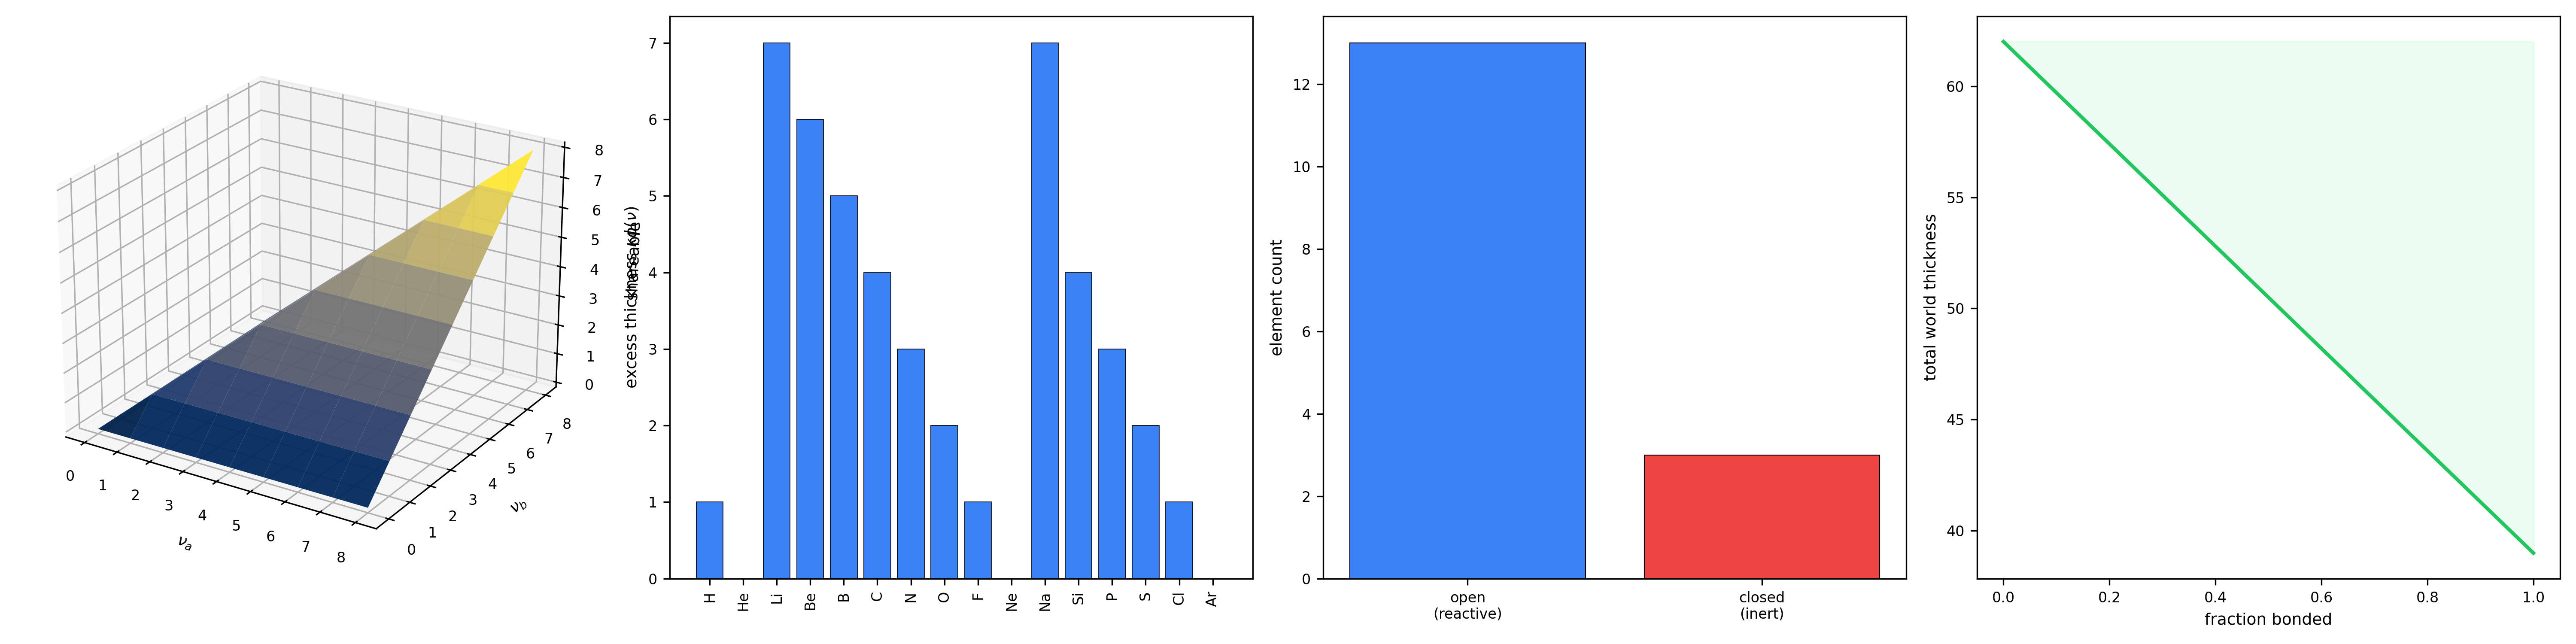
\includegraphics[width=\textwidth]{figures/panel_8_existence.png}
    \caption{\textbf{Why a World of Bounded Atoms Must Be a World of Molecules.}
    (\textbf{A})~Three-dimensional surface of the shareable content $\min(\nu_a,\nu_b)$ over the vacancy plane (cividis): the boundary that two atoms can commit jointly, zero whenever either is closed-shell and rising with the smaller vacancy, the resource from which structure is built.
    (\textbf{B})~Excess boundary thickness $\kappa\phi(\nu)$ above the closed-shell minimum for sixteen elements, bars red where $\nu=0$ (no excess: the noble-gas minimum) and blue where $\nu>0$ (excess to be relaxed by bonding).
    (\textbf{C})~Element census of the open (reactive, blue) versus closed (inert, red) shells among the sixteen elements, the count of atoms that carry shareable vacancy versus those that do not.
    (\textbf{D})~Total world boundary thickness versus the fraction of open atoms that have bonded: the monotone decrease (green, shaded reduction) shows that a world of bounded atoms with positive vacancy lowers its total thickness by forming molecules---chemical structure as the floor's economy (Theorem~\ref{thm:why}).}
    \label{fig:panel_existence}
\end{figure*}
